\documentclass{class}

\usepackage[table]{xcolor}% http://ctan.org/pkg/xcolor
\usetikzlibrary{positioning}
\usepackage{adjustbox}
\usepackage{bbm}
\usepackage{mathrsfs}  
\usepackage{amsmath}% http://ctan.org/pkg/amsmath
\usepackage{tcolorbox}
\setbeamerfont{itemize/enumerate subbody}{size=\normalfont}
\setbeamerfont{itemize/enumerate subsubbody}{size=\normalfont}
\setbeamertemplate{itemize item}{$\bullet$}
\setlength{\leftmargini}{0.25cm}

\title{Self-Selection in Retail Electricity Contracts}
\subtitle{Competition, Regulation, and Welfare Implications}

\author{Léopold Monjoie, Julien Duc}
\institute{Aalto University \and Université Paris Dauphine, PSL Research University}


\apptocmd{\frame}{}{\justifying}{}
\newcommand{\sign}{\text{sign}}
% Conference on Economic Design

\bibliographystyle{apalike}

\begin{document}

\newlength{\tempb}

\frame{\titlepage}

\newcommand{\commentedbox}[2]{%
  \mbox{
    \begin{tabular}[t]{@{}c@{}}
    $\boxed{\displaystyle#1}$\\
    #2
    \end{tabular}%
  }%
}

\newcommand\Wider[2][3em]{%
\makebox[\linewidth][c]{%
  \begin{minipage}{\dimexpr\textwidth+#1\relax}
  \raggedright#2
  \end{minipage}%
  }%
}

\newcommand*\circled[1]{\tikz[baseline=(char.base)]{
            \node[shape=circle,draw,inner sep=2pt] (char) {#1};}}

%%%%%%%%%%%%%%%%%%%%%%%%%%%%%%%%%%%%%%%%%%%%%%%%%%%%%%%%%%%%%%%%%%%%%%%%%%%%%%%%%%%%%%%%%%%%%%%%%%%%%%%%%%%%%%%%%%%%%%%%%%%%%%%%%%%%%%%%%%%%%%%%%%%%%%


\section{Introduction and motivations}


\begin{frame}{Motivations}\label{Motivations}

\begin{mainbox}{Questions}
\begin{itemize}
\vspace{0.15 cm}
    \item  How do heterogeneous consumers self-select into different contracts?
        \vspace{0.15 cm}
    \item How does this sorting interact with retail market equilibrium?
      \vspace{0.15 cm}
    \item Private vs. public provision.
    \vspace{0.15 cm}
\end{itemize}
\end{mainbox}

\vfill

\begin{itemize}    
    \item Focus on \boldrblue{electricity markets}: Fixed Price vs. Dynamic Price contracts. \vfill
    
    \item \boldrblue{First Best.} Consumers should face the (volatile) marginal production cost. \vfill
    
    \item \boldrblue{Moral hazard.} Different contract choices imply allocative inefficiencies.
\end{itemize}

       
\end{frame}

%%%%%%%%%%%%%%%%%%%%%%%%%%%%%%%%%%%%%%%%%%%%%%%%%%%%%%%%%%%%%%%%%%%%%%%%%%%%%%%%%%%%%%%%%%%%%%%%%%%%%%%%%%%%%%%%%%%%%%%%%%%%%%%%%%%%%%%%%%%%%%%%%%%%%%

\begin{frame}{Private contracts coexist with regulated options }\label{UptakeContract2}

\begin{figure}
    \centering
    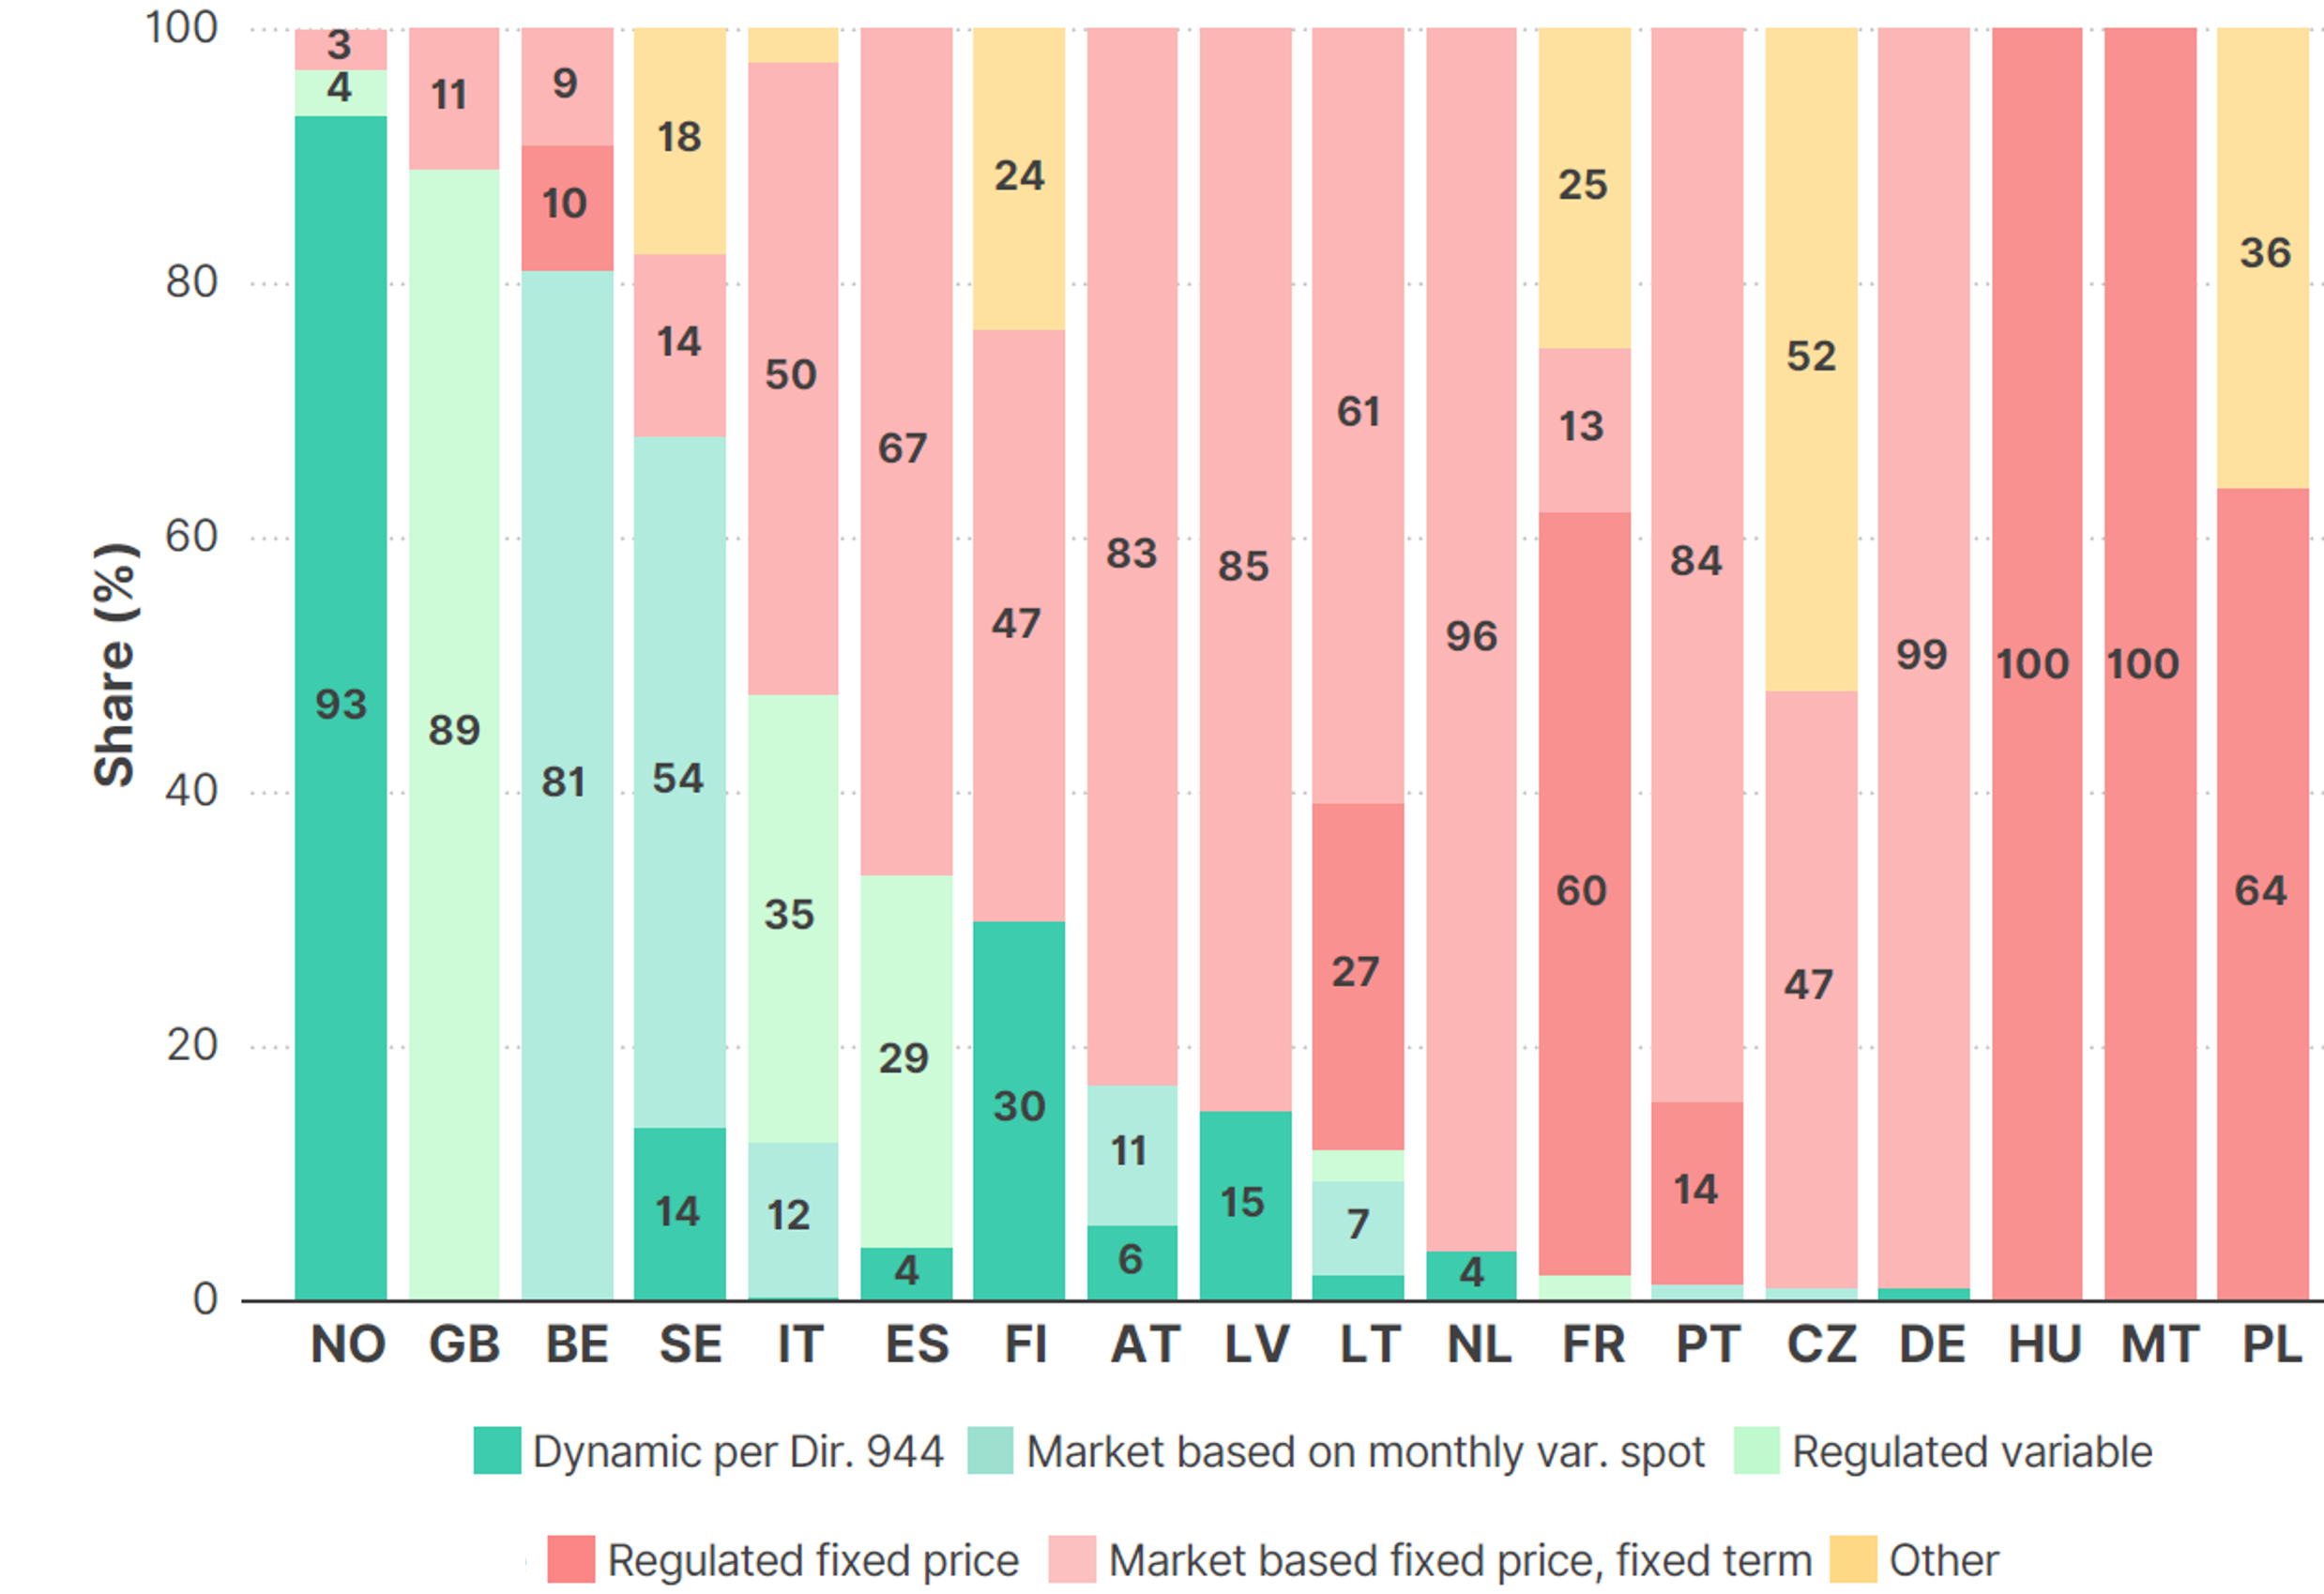
\includegraphics[width=0.8\linewidth]{figure/FP_EU_detail_v2.PNG}
    \caption{Share of household contract uptake in Europe \cite{ACER2024} \hyperlink{options1}{\beamergotobutton{Options}}} 
    \label{fig:FP_EU_detail}
\end{figure}

\end{frame}




%%%%%%%%%%%%%%%%%%%%%%%%%%%%%%%%%%%%%%%%%%%%%%%%%%%%%%%%%%%%%%%%%%%%%%%%%%%%%%%%%%%%%%%%%%%%%%%%%%%%%%%%%%%%%%%%%%%%%%%%%%%%%%%%%%%%%%%%%%%%%%%%%%%%%%



\begin{frame}{First contribution: Demand for contracts with heterogeneous consumers}\label{FirstCont}


\begin{itemize}

\item Provide a \boldrblue{stylized theoretical framework} where a set of consumers have to choose between \boldrblue{a Fixed-Price contract} or \boldrblue{a Dynamic-Price  contract}. \vfill

\begin{itemize}
    \item Extend exogenous share papers. \cite{Borenstein2005b,Leautier2014,Ambec2021,Boom2021}
\end{itemize}

\vfill

\item Consumers consume over \boldrblue{two periods} with \boldrblue{different willingness-to-pay} in each period.
 \vfill

\begin{itemize}
    \item Extend single type consumers model. \cite{joskow2006retail,Astier2021,ancel2025tariffs}
    \item Bundling \cite{Zhou2021} selection markets \cite{Veiga2016}
\end{itemize}

\vfill

\end{itemize}

\begin{mainbox}{Partial Equilibrium}
Provide \boldrblue{the demand} for each contract, given a set of prices and the type of consumers who choose each contract.  
\end{mainbox}


\end{frame}



%%%%%%%%%%%%%%%%%%%%%%%%%%%%%%%%%%%%%%%%%%%%%%%%%%%%%%%%%%%%%%%%%%%%%%%%%%%%%%%%%%%%%%%%%%%%%%%%%%%%%%%%%%%%%%%%%%%%%%%%%%%%%%%%%%%%%%%%%%%%%%%%%%%%%%



\begin{frame}{Second contribution: Market equilibrium with consumer choices}\label{SecondCont}


\begin{itemize}

\item We model \boldrblue{retail competition} between firms that offer the two contracts. 

\vfill

\begin{itemize}
    \item Scarce literature \cite{joskow2006retail}, \cite{Borenstein2003} and \cite{ancel2025tariffs}
\end{itemize}

\vfill

\item Focus on \boldrblue{price equilibrium}.

\vfill

\begin{itemize}
        \item Adverse Selection \cite{1970Akerlof}, price theory \cite{Einav2012}, competition \cite{Azevedo2017}
\end{itemize}
    
\vfill

\item The \boldrblue{market} is composed of private retailers and a regulated firm.


\vfill

\begin{itemize}
\item Regulation theory \cite{laffont1993theory}, public vs private options \cite{Martimort2020a,Kang2023a}.
\end{itemize}
\end{itemize}


\vfill

\begin{mainbox}{General Equilibrium}
We characterize \boldrblue{the price and welfare equilibrium} in the retail market when consumers can self-select.
\end{mainbox}

\end{frame}



%%%%%%%%%%%%%%%%%%%%%%%%%%%%%%%%%%%%%%%%%%%%%%%%%%%%%%%%%%%%%%%%%%%%%%%%%%%%%%%%%%%%%%%%%%%%%%%%%%%%%%%%%%%%%%%%%%%%%%%%%%%%%%%%%%%%%%%%%%%%%%%%%%%%%%

\begin{frame}{Main takeaways}


\begin{itemize}

\item \boldrblue{A selection model}. heterogeneity and multidimensionality of types $\rightarrow$ retail cost depends on consumer types and contract choices.


\vfill

\item \boldrblue{Optimal demand for contracts}: Higher willingness to pay during low-price periods $\rightarrow$ dynamic contract. Opposite for the fixed-price contract.

\vfill

\item \boldrblue{Market equilibrium}.

\vfill

\begin{itemize}
    \item In the equilibrium, only a public firm may offer a fixed-price contract. \vfill

\item \boldrblue{Adverse selection}: \vfill

    \begin{center}
    $W$(\textcolor{blue}{Private} / \textcolor{blue}{Dynamic} + \textcolor{red}{Public} / \textcolor{red}{Fixed-Price})  { \textbf{  < }} $W$( \textcolor{red}{Fixed-Price})
   \end{center}

\vfill

\item Leakage of consumers to the private firms $\rightarrow$ low equilibrium fixed-price.

    \end{itemize}

\end{itemize}


\end{frame}


%%%%%%%%%%%%%%%%%%%%%%%%%%%%%%%%%%%%%%%%%%%%%%%%%%%%%%%%%%%%%%%%%%%%%%%%%%%%%%%%%%%%%%%%%%%%%%%%%%%%%%%%%%%%%%%%%%%%%%%%%%%%%%%%%%%%%%%%%%%%%%%%%%%%%%
%%%%%%%%%%%%%%%%%%%%%%%%%%%%%%%%%%%%%%%%%%%%%%%%%%%%%%%%%%%%%%%%%%%%%%%%%%%%%%%%%%%%%%%%%%%%%%%%%%%%%%%%%%%%%%%%%%%%%%%%%%%%%%%%%%%%%%%%%%%%%%%%%%%%%%
%%%%%%%%%%%%%%%%%%%%%%%%%%%%%%%%%%%%%%%%%%%%%%%%%%%%%%%%%%%%%%%%%%%%%%%%%%%%%%%%%%%%%%%%%%%%%%%%%%%%%%%%%%%%%%%%%%%%%%%%%%%%%%%%%%%%%%%%%%%%%%%%%%%%%%

\section{The model}

% \subsection{The environment}

\begin{frame}{Roadmap}
  \tableofcontents [sectionstyle=show/shaded,subsectionstyle=show/shaded]
\end{frame}


%%%%%%%%%%%%%%%%%%%%%%%%%%%%%%%%%%%%%%%%%%%%%%%%%%%%%%%%%%%%%%%%%%%%%%%%%%%%%%%%%%%%%%%%%%%%%%%%%%%%%%%%%%%%%%%%%%%%%%%%%%%%%%%%%%%%%%%%%%%%%%%%%%%%%%


\begin{frame}{Timing}


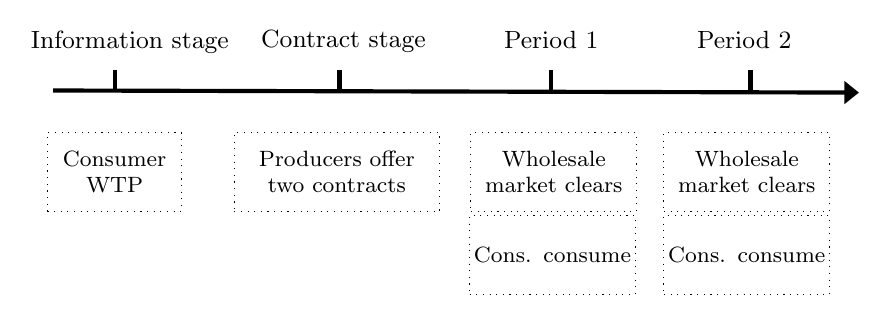
\begin{tikzpicture}[x=0.45pt,y=0.75pt,yscale=-1,xscale=1]

\draw [line width=1.5]    (20,100) -- (663,101) ;
\draw [shift={(667,101)}, rotate = 180.07] [fill={rgb, 255:red, 0; green, 0; blue, 0 }  ][line width=0.08]  [draw opacity=0] (11.61,-5.58) -- (0,0) -- (11.61,5.58) -- cycle    ;
\draw [line width=1.5,color = black]    (70,90) -- (70,100) ;
\draw [line width=1.5,color = black]   (250,90) -- (250,100) ;
\draw [line width=1.5,color = black]   (420,90) -- (420,100)  ;
\draw [line width=1.5,color = black]    (580,90) -- (580,100)   ;

% Text Node
\draw (0,70) node [anchor=north west][inner sep=0.75pt]  [font=\small] [align=center] {Information stage};
\draw (185,70) node [anchor=north west][inner sep=0.75pt]  [font=\small] [align=center] {Contract  stage};
\draw (380,70) node [anchor=north west][inner sep=0.75pt]  [font=\small] [align=center] {Period 1};
\draw (535,70) node [anchor=north west][inner sep=0.75pt]  [font=\small] [align=center] {Period 2};

\draw (15,120) node [draw = black,anchor=north west,minimum height = 1 cm,  text  width = 1.6cm][inner sep=1.5pt,dotted]  [font=\footnotesize] [align=center] {Consumer WTP};
% \draw (15,160) node [anchor=north west,minimum height = 1 cm,  text  width = 1.6cm,dotted][inner sep=1.5pt]  [font=\footnotesize] [align=center] { \textit{common info.} \\ \textit{private info.}};

\draw (165,120) node [draw = black,anchor=north west,minimum height = 1 cm,  text  width = 2.5cm][inner sep=1.5pt,dotted]  [font=\footnotesize] [align=center]{ Producers offer \\ two contracts};
\draw (355,120) node [draw = black,anchor=north west,minimum height = 1 cm,  text  width =  2cm,dotted][inner sep=1.5pt]  [font=\footnotesize] [align=center] { Wholesale  \\ market clears};
\draw (354,160) node [draw = black,anchor=north west,minimum height = 1 cm,  text  width = 2cm,dotted][inner sep=1.5pt]  [font=\footnotesize] [align=center] { Cons. consume};

\draw (510,120) node [draw = black,anchor=north west,minimum height = 1 cm,  text  width = 2cm,dotted][inner sep=1.5pt]  [font=\footnotesize] [align=center] { Wholesale  \\ market clears};
\draw (510,160) node [draw = black,anchor=north west,minimum height = 1 cm,  text  width = 2cm,dotted][inner sep=1.5pt]  [font=\footnotesize] [align=center] { Cons. consume};

\end{tikzpicture}

    
\end{frame}



%%%%%%%%%%%%%%%%%%%%%%%%%%%%%%%%%%%%%%%%%%%%%%%%%%%%%%%%%%%%%%%%%%%%%%%%%%%%%%%%%%%%%%%%%%%%%%%%%%%%%%%%%%%%%%%%%%%%%%%%%%%%%%%%%%%%%%%%%%%%%%%%%%%%%%

\begin{frame}{Consumers}

\begin{itemize}
    \item A unit mass of consumers.

\vfill

    \item With a \boldrblue{unit demand} for electricity for each two periods $t = 1,2$.

\vfill

    \item W.t.p: a \boldrblue{two-dimensional} type $\textbf{v}=(v_1,v_2) $
    
\vfill

        % \begin{itemize}
 \item Drawn from a pdf. $f_t(v)$ and cdf. $F_t(v)$ with support $[\underline{v}_t,\bar{v}_t]$. 
            
% \vfill

        % \item Even though the distributions are independent, we assume the affine relationship between the two periods, where $\alpha,\beta \in \mathbb{R}$.

% \end{itemize}

        % \begin{equation*}
        %     [ \ubar{v}_2, \bar{v}_2] = [\alpha + \beta \ubar{v}_1, \alpha + \beta \bar{v}_1]
        % \end{equation*}


\vfill

\item Type $\textbf{v}$ consumer surplus from consuming at price profile $\textbf{p}$ is:

\begin{equation*}
 u\left(\textbf{v},\textbf{p}\right)= v_1-p_1 +  v_2-p_2
 \end{equation*}
\end{itemize}    
\end{frame}

%%%%%%%%%%%%%%%%%%%%%%%%%%%%%%%%%%%%%%%%%%%%%%%%%%%%%%%%%%%%%%%%%%%%%%%%%%%%%%%%%%%%%%%%%%%%%%%%%%%%%%%%%%%%%%%%%%%%%%%%%%%%%%%%%%%%%%%%%%%%%%%%%%%%%%

\begin{frame}{Wholesale market}


\begin{itemize}
    \item \boldrblue{Perfectly competitive firms} produce each periods $q$ unit of electricity at a linear production cost: 
\end{itemize}

\begin{equation*}
    C_t(q) = c_t q
\end{equation*}

\vfill

\begin{itemize}
    \item We assume w.l.o.g. that $c_1 < c_2$

\vfill

\begin{itemize}
    \item Off-peak period: $t = 1$ and On-peak period: $t = 2$. \vfill
    \item Due to perfect competition: $\textbf{p}_w = \{p_1^w,p_2^w\} = \{c_1,c_2\}$.
\end{itemize}

\vfill

\item Period 1 is a sunny afternoon with renewable production with null marginal cost, and period 2 is the evening with fuel producers with high marginal cost.


\vfill

\item  No uncertainty, no investment decision, and no capacity constraints.

\end{itemize}
    
\end{frame}

%%%%%%%%%%%%%%%%%%%%%%%%%%%%%%%%%%%%%%%%%%%%%%%%%%%%%%%%%%%%%%%%%%%%%%%%%%%%%%%%%%%%%%%%%%%%%%%%%%%%%%%%%%%%%%%%%%%%%%%%%%%%%%%%%%%%%%%%%%%%%%%%%%%%%%

\begin{frame}{Retailers}

\begin{itemize}
    \item We assume a set of retailers that purchase at no cost on the wholesale market.

    \vfill

    \item We take the characteristics of contracts and the set of contracts as given.  \vfill
    
    \item If $\textbf{p}_k=(p_1^k,p_2^k)$ is profile unit-price of contract $k$, then:  \vfill

    \begin{itemize}
        \item FP contract: $\textbf{p}_{r} =  (p_r,p_r)$ \vfill
        \item Dynamic contract: $\textbf{p}_{s} =  (p_1,p_2)$
    \end{itemize}

\end{itemize}


    
\end{frame}

%%%%%%%%%%%%%%%%%%%%%%%%%%%%%%%%%%%%%%%%%%%%%%%%%%%%%%%%%%%%%%%%%%%%%%%%%%%%%%%%%%%%%%%%%%%%%%%%%%%%%%%%%%%%%%%%%%%%%%%%%%%%%%%%%%%%%%%%%%%%%%%%%%%%%%


\begin{frame}{Equilibrium Definition}


\begin{itemize}

\item The optimal consumer choose a consumption profile $\textbf{x} = (x_1,x_2)$ with $x_t =\{0,1\}$, given a contract, to maximize its utility:

\vfill

\begin{equation*}
U\left(\textbf{v},\textbf{p}_k\right) \quad = \quad  \max_{\textbf{x}} \quad \textbf{x} (\textbf{v} - \textbf{p}_k) 
\end{equation*}

\vfill
    
\item Given a contract $k$, a \textit{private firm} equilibrium is such that:

\vfill

\begin{equation*}
 \pi_k(\textbf{p}_{k}) = \textbf{q}_k (\textbf{p}_k - \textbf{p}_w)  =0 
\end{equation*}

\vfill

\item We restrict the \textit{public firm} to offer the fixed-price contract and the equilibrium is such that:

\vfill

\begin{equation*}
 \max \quad CS^r(\textbf{p}_r) + (1+\lambda)\pi_r(\textbf{p}_{r})
\end{equation*}

\end{itemize}

{\footnotesize $\mu_k = $ mass of consumers}
    
\end{frame}
%%%%%%%%%%%%%%%%%%%%%%%%%%%%%%%%%%%%%%%%%%%%%%%%%%%%%%%%%%%%%%%%%%%%%%%%%%%%%%%%%%%%%%%%%%%%%%%%%%%%%%%%%%%%%%%%%%%%%%%%%%%%%%%%%%%%%%%%%%%%%%%%%%%%%%


% \begin{frame}{Example with one contract}
% \begin{figure}
%     \centering
%     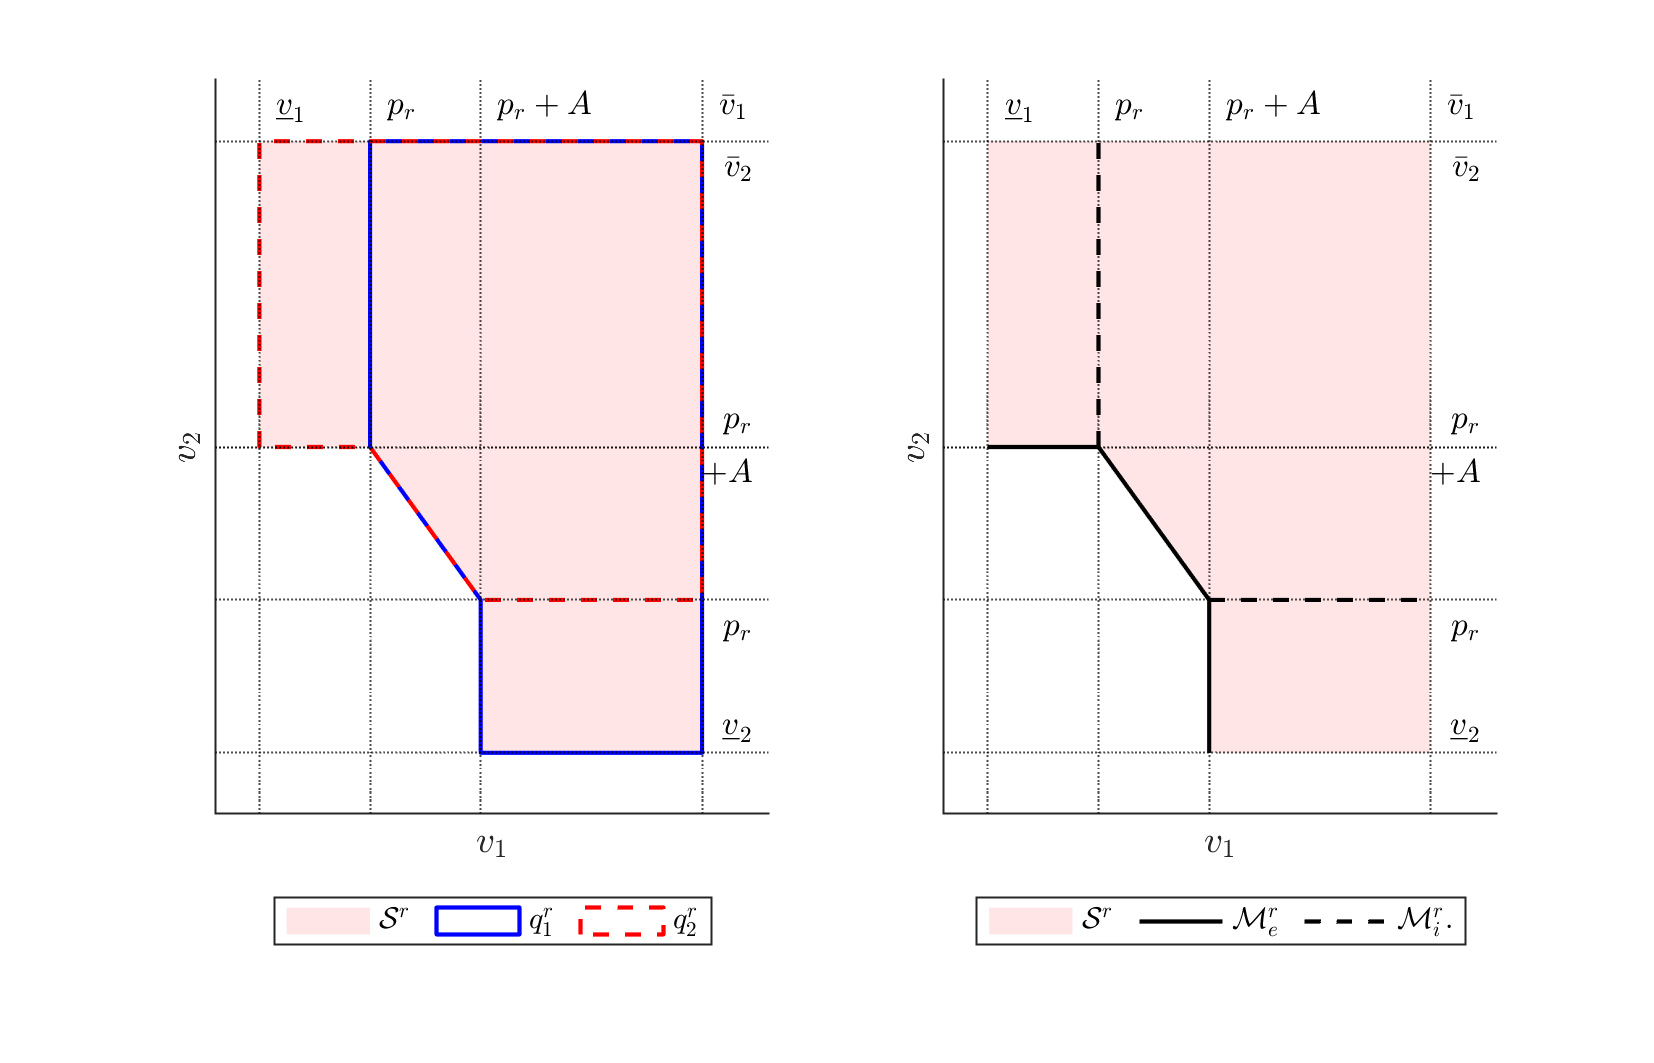
\includegraphics[width=1\linewidth]{figure/intro_zone_A_ppt.png}
%     \caption{Demand for the fixed-price contract, and marginal consumers (\textit{exiters and profile switchers}).}
%     \label{fig:intro_zone_mu}
% \end{figure}


% \end{frame}
% %%%%%%%%%%%%%%%%%%%%%%%%%%%%%%%%%%%%%%%%%%%%%%%%%%%%%%%%%%%%%%%%%%%%%%%%%%%%%%%%%%%%%%%%%%%%%%%%%%%%%%%%%%%%%%%%%%%%%%%%%%%%%%%%%%%%%%%%%%%%%%%%%%%%%%

% \begin{frame}{Single Contract Equilibrium}

% \begin{itemize}

%  \item If private retailers offer the FP contract, then the linear price is the eq. and takes the following form:

% \begin{equation*}
%  p_r^* =  \text{av. total cost}   \quad \text{and} \quad A_r^* =0 
% \end{equation*}

% \vfill

% \item If private retailers offer the RTP contract, then competition implies full cost pass-through to consumers:

% \vfill

% \begin{equation*}
%  \textbf{p}_s^*  = \{p_1^w,p_2^w\}  = \{c_1,c_2\}   \quad \text{and} \quad A_s^* =0 
% \end{equation*}

% \vfill

% \item If the regulated monopoly offers the FP contract, then: 

% \vfill

%         \begin{equation*}
%             p_r^{**} \quad = \quad \text{av.marg.cost} \quad + \quad \text{ramsey A}  \quad- \quad \underbrace{\bigg.A^{**}_r \frac{\delta_A\mu_r}{\delta_A q^r} \bigg.}_{\text{switchers wedge}}
%         \end{equation*}



% \end{itemize}

% \end{frame}

%%%%%%%%%%%%%%%%%%%%%%%%%%%%%%%%%%%%%%%%%%%%%%%%%%%%%%%%%%%%%%%%%%%%%%%%%%%%%%%%%%%%%%%%%%%%%%%%%%%%%%%%%%%%%%%%%%%%%%%%%%%%%%%%%%%%%%%%%%%%%%%%%%%%%%

% \begin{frame}{Adverse Selection in Single Contract Equilibrium}

% \begin{itemize}

% \item We derive sufficient and necessary conditions for the private and public equilibrium to exhibit adverse (or advantageous) selection.  \vfill

% \item  Private equilibrium (sufficient conditions):   \vfill

% \begin{equation*}
%  \frac{\# \text{marginal cons. in 1}}{\# \text{ cons. in 1}} > \frac{\# \text{marginal cons. in 2}}{\# \text{ cons. in 2}}   
% \end{equation*}

% \vfill

% \item  Public equilibrium (necessary conditions):   \vfill

% \begin{equation*}
%  \frac{\# \text{profile switchers in 1}}{\# \text{ cons. in 1}} <  (>)  \frac{\# \text{profile switchers in 2}}{\# \text{cons. in 2}}   \quad \text{and} \quad \lambda > (<)1 
% \end{equation*}

% \end{itemize}

% \end{frame}


\begin{frame}{The single contract case}

\begin{figure}
    \centering
    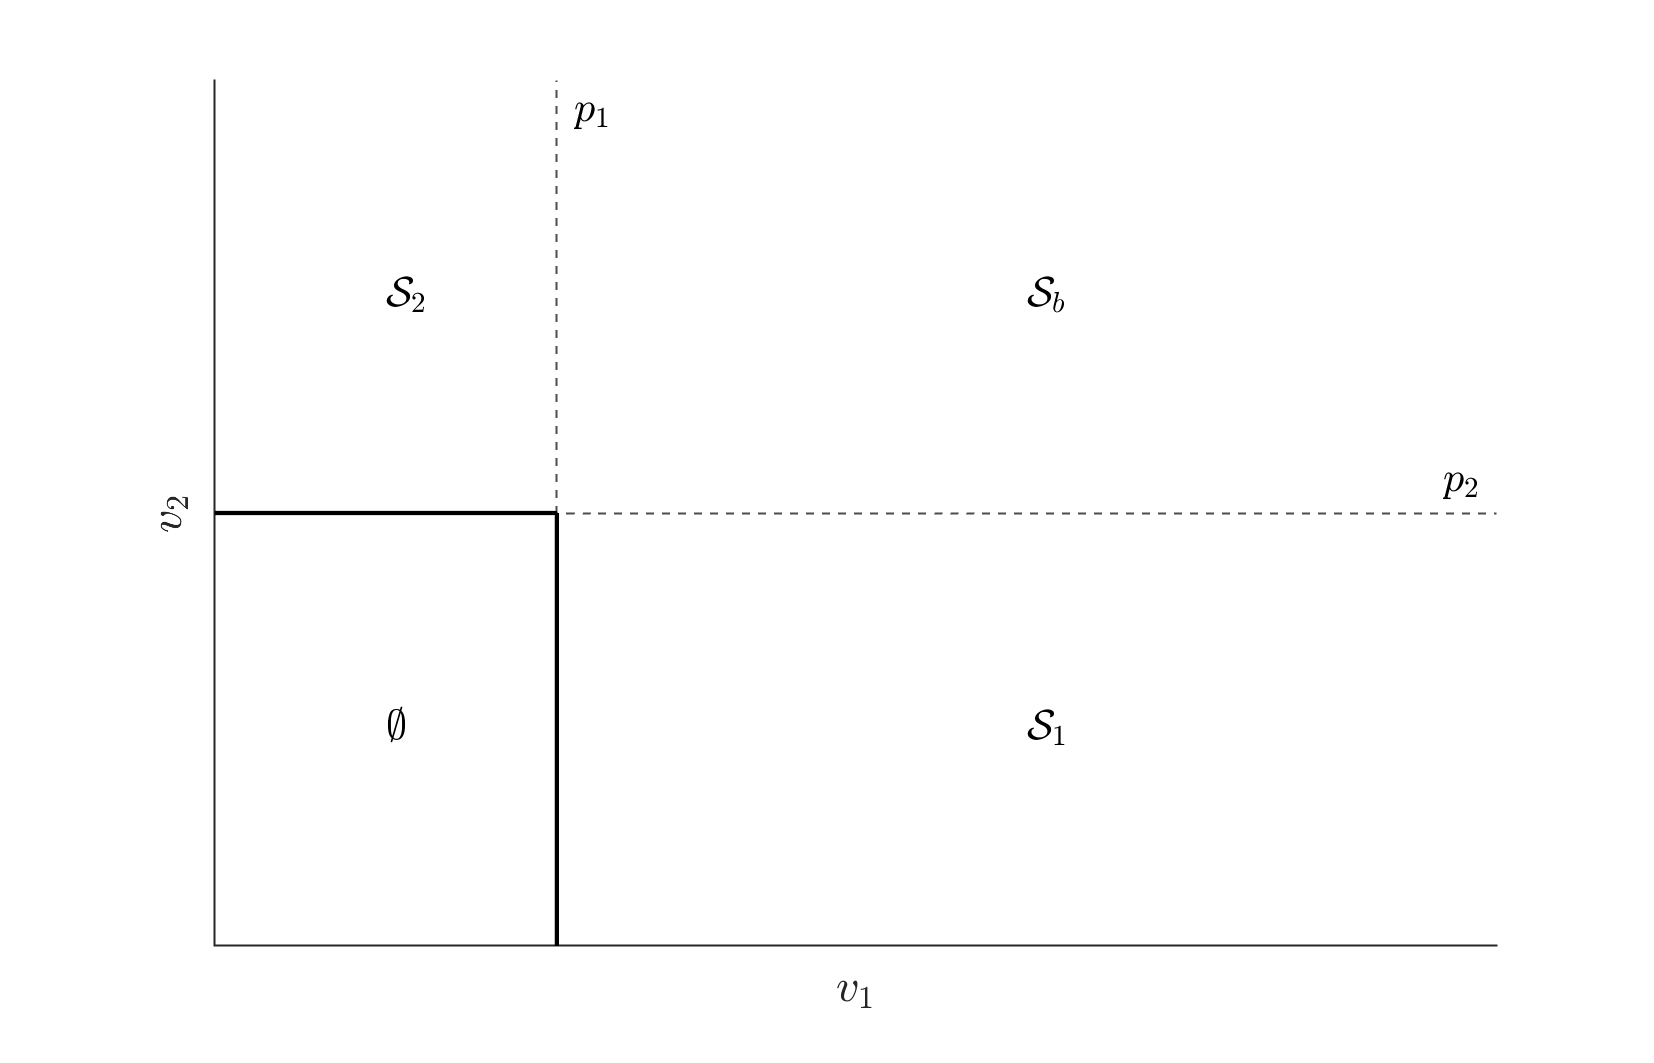
\includegraphics[width=0.8\linewidth]{figure/spot_demand_multi.png}
     \caption{The canonical bundle case.} 
    \label{fig:spot_demand_multi}
\end{figure}
    
    
\end{frame}
%%%%%%%%%%%%%%%%%%%%%%%%%%%%%%%%%%%%%%%%%%%%%%%%%%%%%%%%%%%%%%%%%%%%%%%%%%%%%%%%%%%%%%%%%%%%%%%%%%%%%%%%%%%%%%%%%%%%%%%%%%%%%%%%%%%%%%%%%%%%%%%%%%%%%%
%%%%%%%%%%%%%%%%%%%%%%%%%%%%%%%%%%%%%%%%%%%%%%%%%%%%%%%%%%%%%%%%%%%%%%%%%%%%%%%%%%%%%%%%%%%%%%%%%%%%%%%%%%%%%%%%%%%%%%%%%%%%%%%%%%%%%%%%%%%%%%%%%%%%%%
%%%%%%%%%%%%%%%%%%%%%%%%%%%%%%%%%%%%%%%%%%%%%%%%%%%%%%%%%%%%%%%%%%%%%%%%%%%%%%%%%%%%%%%%%%%%%%%%%%%%%%%%%%%%%%%%%%%%%%%%%%%%%%%%%%%%%%%%%%%%%%%%%%%%%%

\section{Partial equilibrium: Demand for multiple contracts}


\begin{frame}{Roadmap}
  \tableofcontents [sectionstyle=show/shaded,subsectionstyle=show/shaded]
\end{frame}



%%%%%%%%%%%%%%%%%%%%%%%%%%%%%%%%%%%%%%%%%%%%%%%%%%%%%%%%%%%%%%%%%%%%%%%%%%%%%%%%%%%%%%%%%%%%%%%%%%%%%%%%%%%%%%%%%%%%%%%%%%%%%%%%%%%%%%%%%%%%%%%%%%%%%%



\begin{frame}{The marginal consumers}


\begin{itemize}

\item Partial equilibrium: contract prices as given: $p_1 < p_r < p_2$ \vfill


\item Marginal consumers $\equiv $ same utility over at least two options when optimizing over the set of contracts and consumption profiles.

\vfill

\item There are three types

\vfill

\begin{itemize}
    \item \textit{Exiters} - stop consuming \vfill
    \item \textit{Profile switchers} - 2 periods vs 1 period in the same contract \vfill
    \item Contract switchers - switch contract and consumption profile 
\end{itemize}



\end{itemize}

\end{frame}

%%%%%%%%%%%%%%%%%%%%%%%%%%%%%%%%%%%%%%%%%%%%%%%%%%%%%%%%%%%%%%%%%%%%%%%%%%%%%%%%%%%%%%%%%%%%%%%%%%%%%%%%%%%%%%%%%%%%%%%%%%%%%%%%%%%%%%%%%%%%%%%%%%%%%%


\begin{frame}{Illustration}\label{PlotIndifConso}

\begin{figure}
    \centering
    \includegraphics[width=1\linewidth]{figure/example_cstc_ppt.png}
     \caption{Contract switchers are defined by the red lines.} 
    \label{fig:example_conv_cstc_nocol}
\end{figure}
    
\end{frame}


%%%%%%%%%%%%%%%%%%%%%%%%%%%%%%%%%%%%%%%%%%%%%%%%%%%%%%%%%%%%%%%%%%%%%%%%%%%%%%%%%%%%%%%%%%%%%%%%%%%%%%%%%%%%%%%%%%%%%%%%%%%%%%%%%%%%%%%%%%%%%%%%%%%%%%

\begin{frame}{The demand for contracts}\label{ExogenousDemand}

\begin{figure}
    \centering
    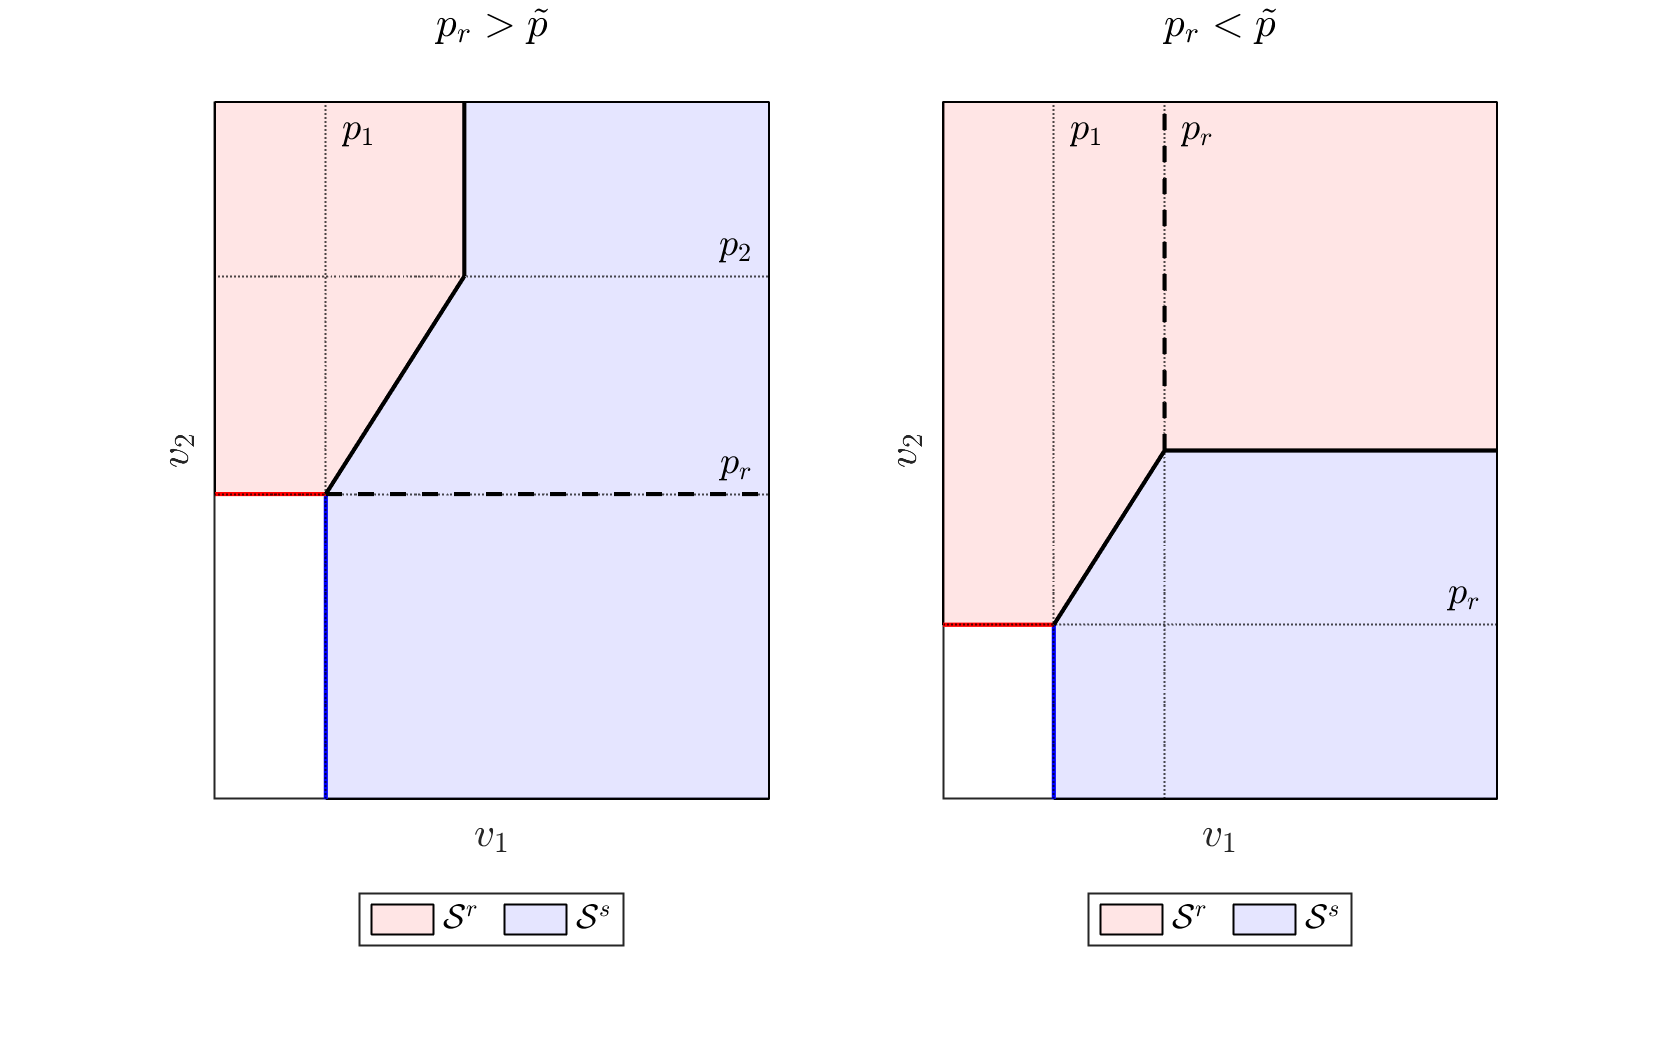
\includegraphics[width=1\linewidth]{figure/example_conv_cstc_ppt.png}
     \caption{The set of \textit{contract switchers} defines the mass of consumers choosing each contract.}
\end{figure}
    
\end{frame}


% \begin{frame}{Implication 2: The demand for electricity}\label{ExogenousDemand}

% \begin{figure}
%     \centering
%     \includegraphics[width=1\linewidth]{figure/example_conv_cqtt.png}
%      \caption{When $p_r < \Tilde{p}$ (resp. $p_r > \tilde{p}$ ), some consumers that choose the FP contract (resp. RTP contract) consume in both periods, while consumers under the RTP contracts (resp. FP contract) consume only during period 1 (resp. period 2).}
%     \label{fig:example_conv_cstc4}
% \end{figure}
    
% \end{frame}


%%%%%%%%%%%%%%%%%%%%%%%%%%%%%%%%%%%%%%%%%%%%%%%%%%%%%%%%%%%%%%%%%%%%%%%%%%%%%%%%%%%%%%%%%%%%%%%%%%%%%%%%%%%%%%%%%%%%%%%%%%%%%%%%%%%%%%%%%%%%%%%%%%%%%%
%%%%%%%%%%%%%%%%%%%%%%%%%%%%%%%%%%%%%%%%%%%%%%%%%%%%%%%%%%%%%%%%%%%%%%%%%%%%%%%%%%%%%%%%%%%%%%%%%%%%%%%%%%%%%%%%%%%%%%%%%%%%%%%%%%%%%%%%%%%%%%%%%%%%%%
%%%%%%%%%%%%%%%%%%%%%%%%%%%%%%%%%%%%%%%%%%%%%%%%%%%%%%%%%%%%%%%%%%%%%%%%%%%%%%%%%%%%%%%%%%%%%%%%%%%%%%%%%%%%%%%%%%%%%%%%%%%%%%%%%%%%%%%%%%%%%%%%%%%%%%

\section{General equilibrium: Retail prices}

\begin{frame}{Roadmap}
  \tableofcontents [sectionstyle=show/shaded,subsectionstyle=show/shaded]
\end{frame}

%%%%%%%%%%%%%%%%%%%%%%%%%%%%%%%%%%%%%%%%%%%%%%%%%%%%%%%%%%%%%%%%%%%%%%%%%%%%%%%%%%%%%%%%%%%%%%%%%%%%%%%%%%%%%%%%%%%%%%%%%%%%%%%%%%%%%%%%%%%%%%%%%%%%%%

\begin{frame}{Incentives for fixed-price contract}

\begin{figure}
    \centering
    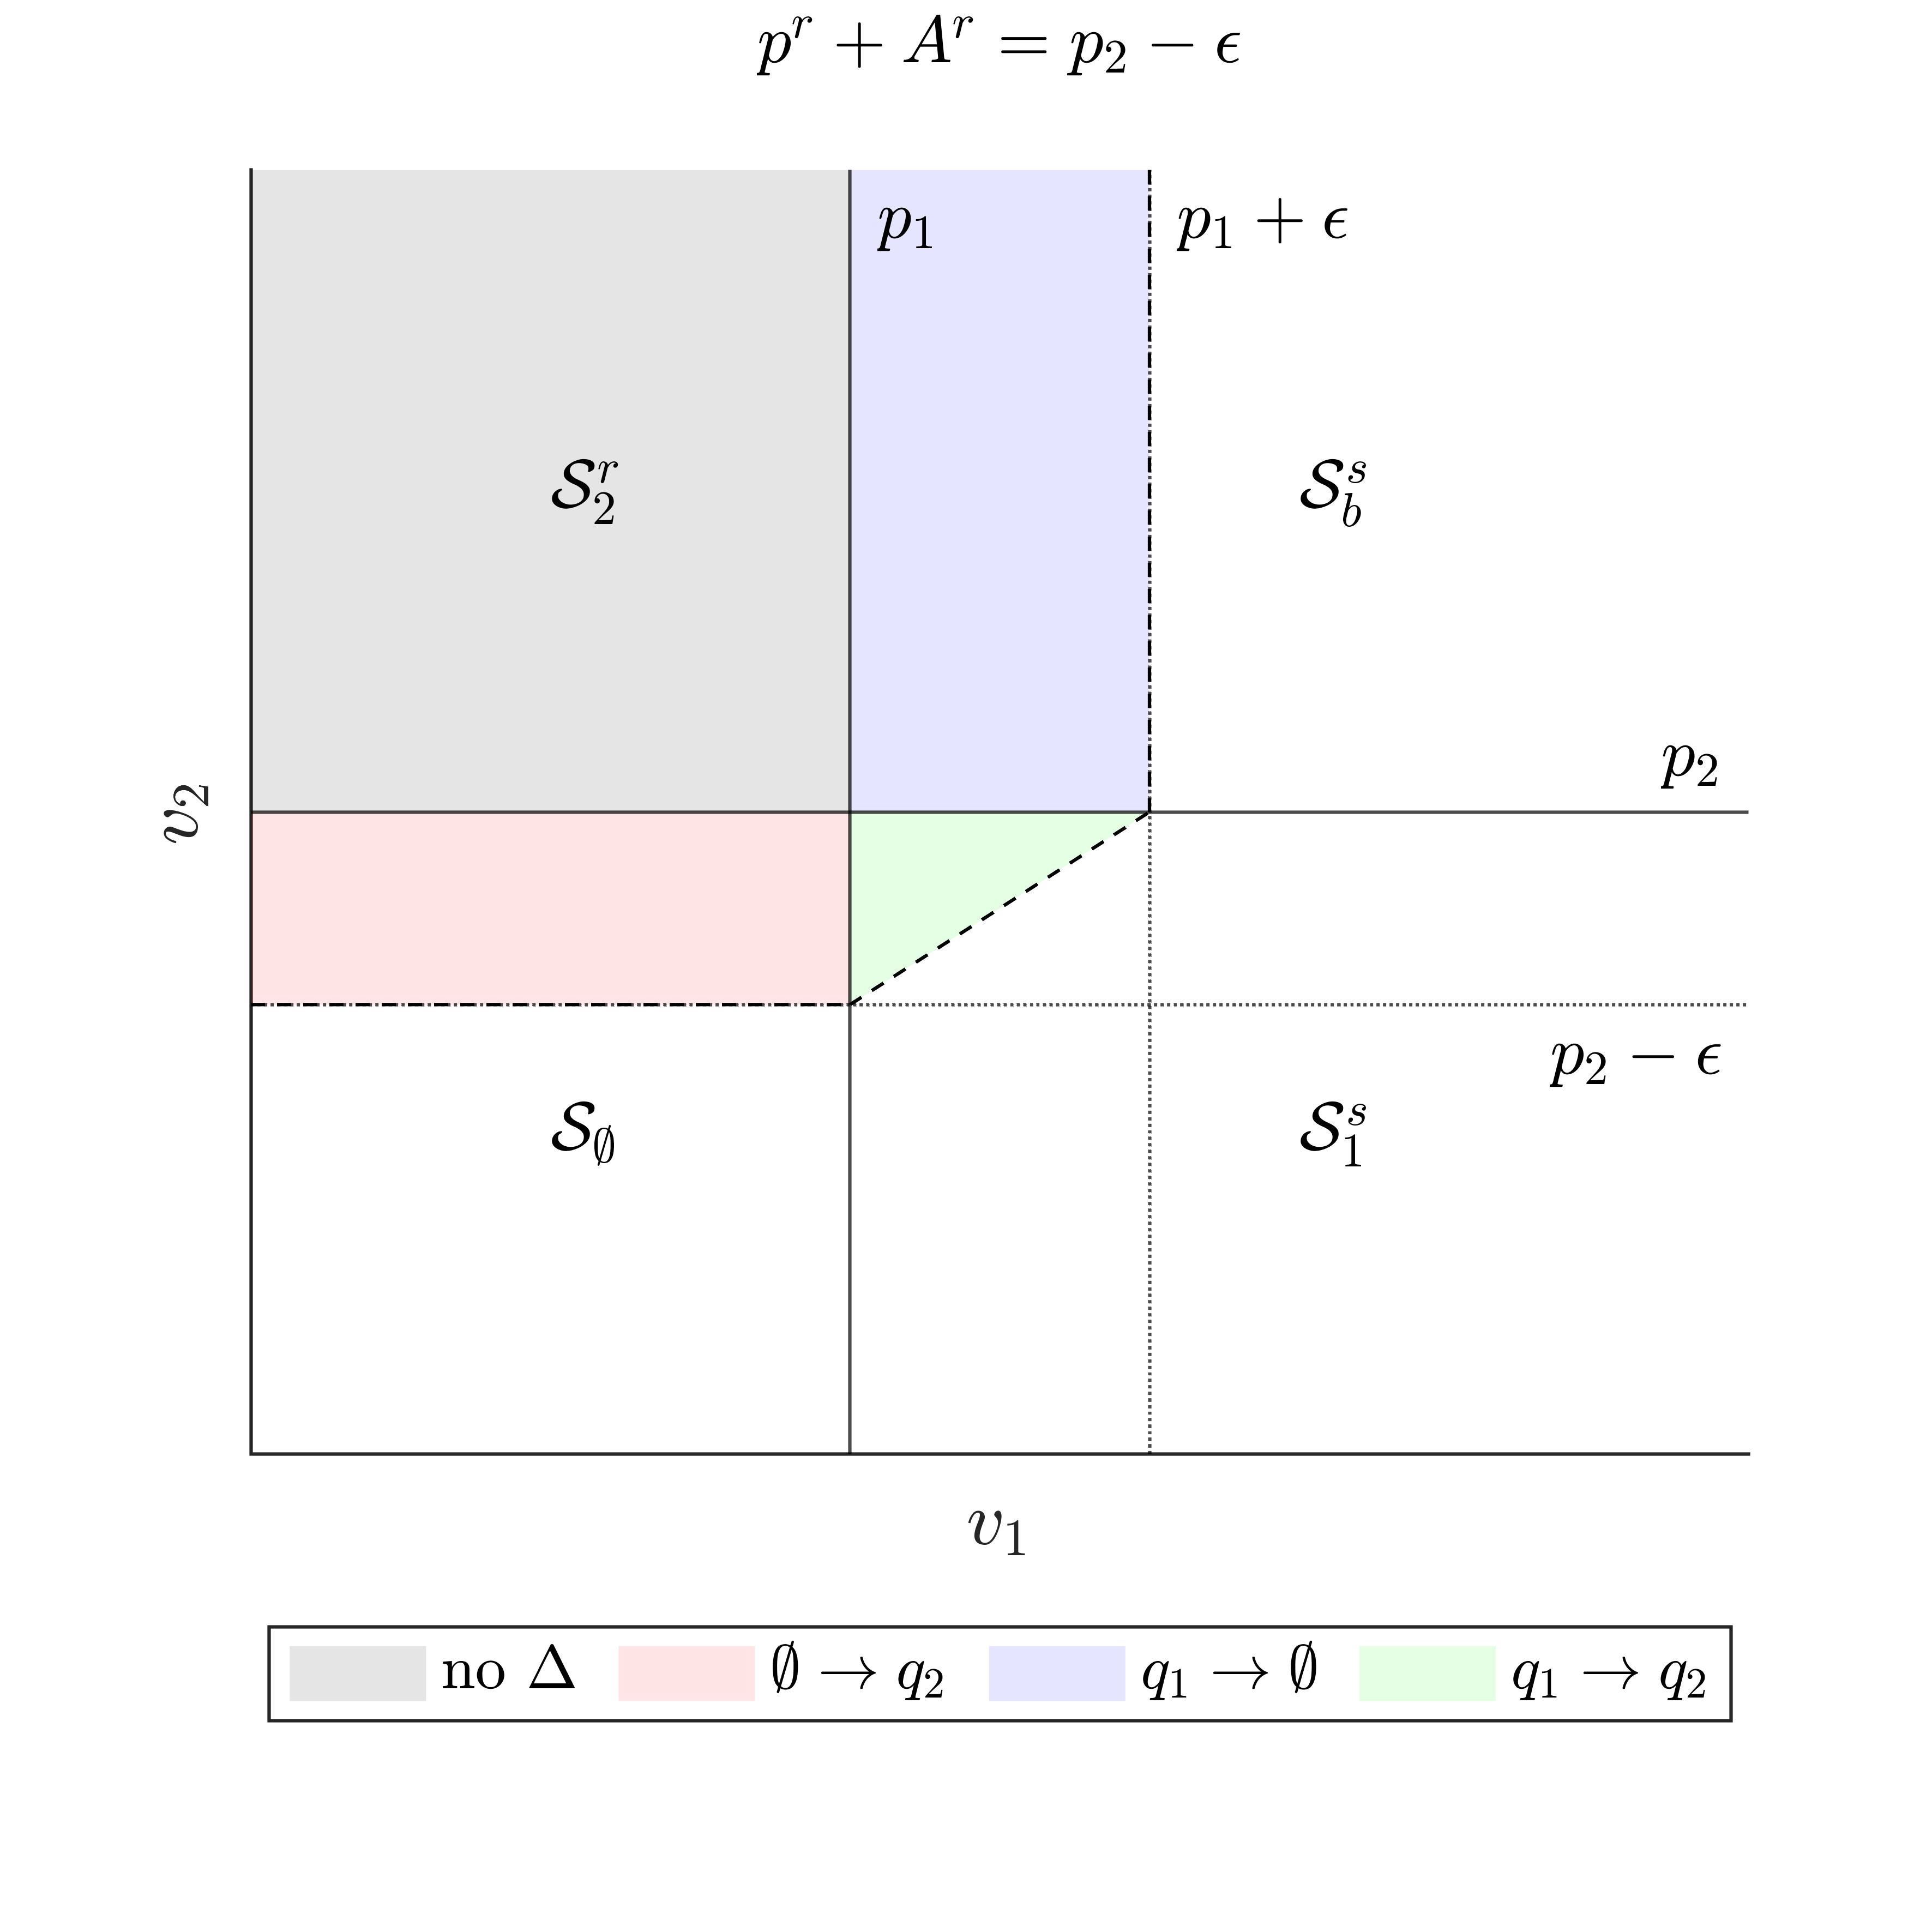
\includegraphics[width=1\linewidth]{figure/spot_demand_multi_sb_ppt.png}
    \caption{Downward price deviation of the fixed price with entry.}
    \label{fig:spot_demand_multi_sb_ppt}
\end{figure}
    
\end{frame}

%%%%%%%%%%%%%%%%%%%%%%%%%%%%%%%%%%%%%%%%%%%%%%%%%%%%%%%%%%%%%%%%%%%%%%%%%%%%%%%%%%%%%%%%%%%%%%%%%%%%%%%%%%%%%%%%%%%%%%%%%%%%%%%%%%%%%%%%%%%%%%%%%%%%%%

\begin{frame}{Private Firms only offer dynamic contracts in equilibrium}\label{PrivateFirms2}


\begin{claim}
 With private firms, the equilibrium prices of the dynamic contract are equal to the wholesale market prices.
\end{claim}

\vfill

\begin{proposition}
 With private firms, there is no equilibrium with consumers having a strict preference for the fixed-price contract. 
\end{proposition}


\end{frame}
% 
%%%%%%%%%%%%%%%%%%%%%%%%%%%%%%%%%%%%%%%%%%%%%%%%%%%%%%%%%%%%%%%%%%%%%%%%%%%%%%%%%%%%%%%%%%%%%%%%%%%%%%%%%%%%%%%%%%%%%%%%%%%%%%%%%%%%%%%%%%%%%%%%%%%%%%

\begin{frame}{Market unraveling of the fixed-price market} \label{PrivateFirms2}


\begin{figure}
    \centering
    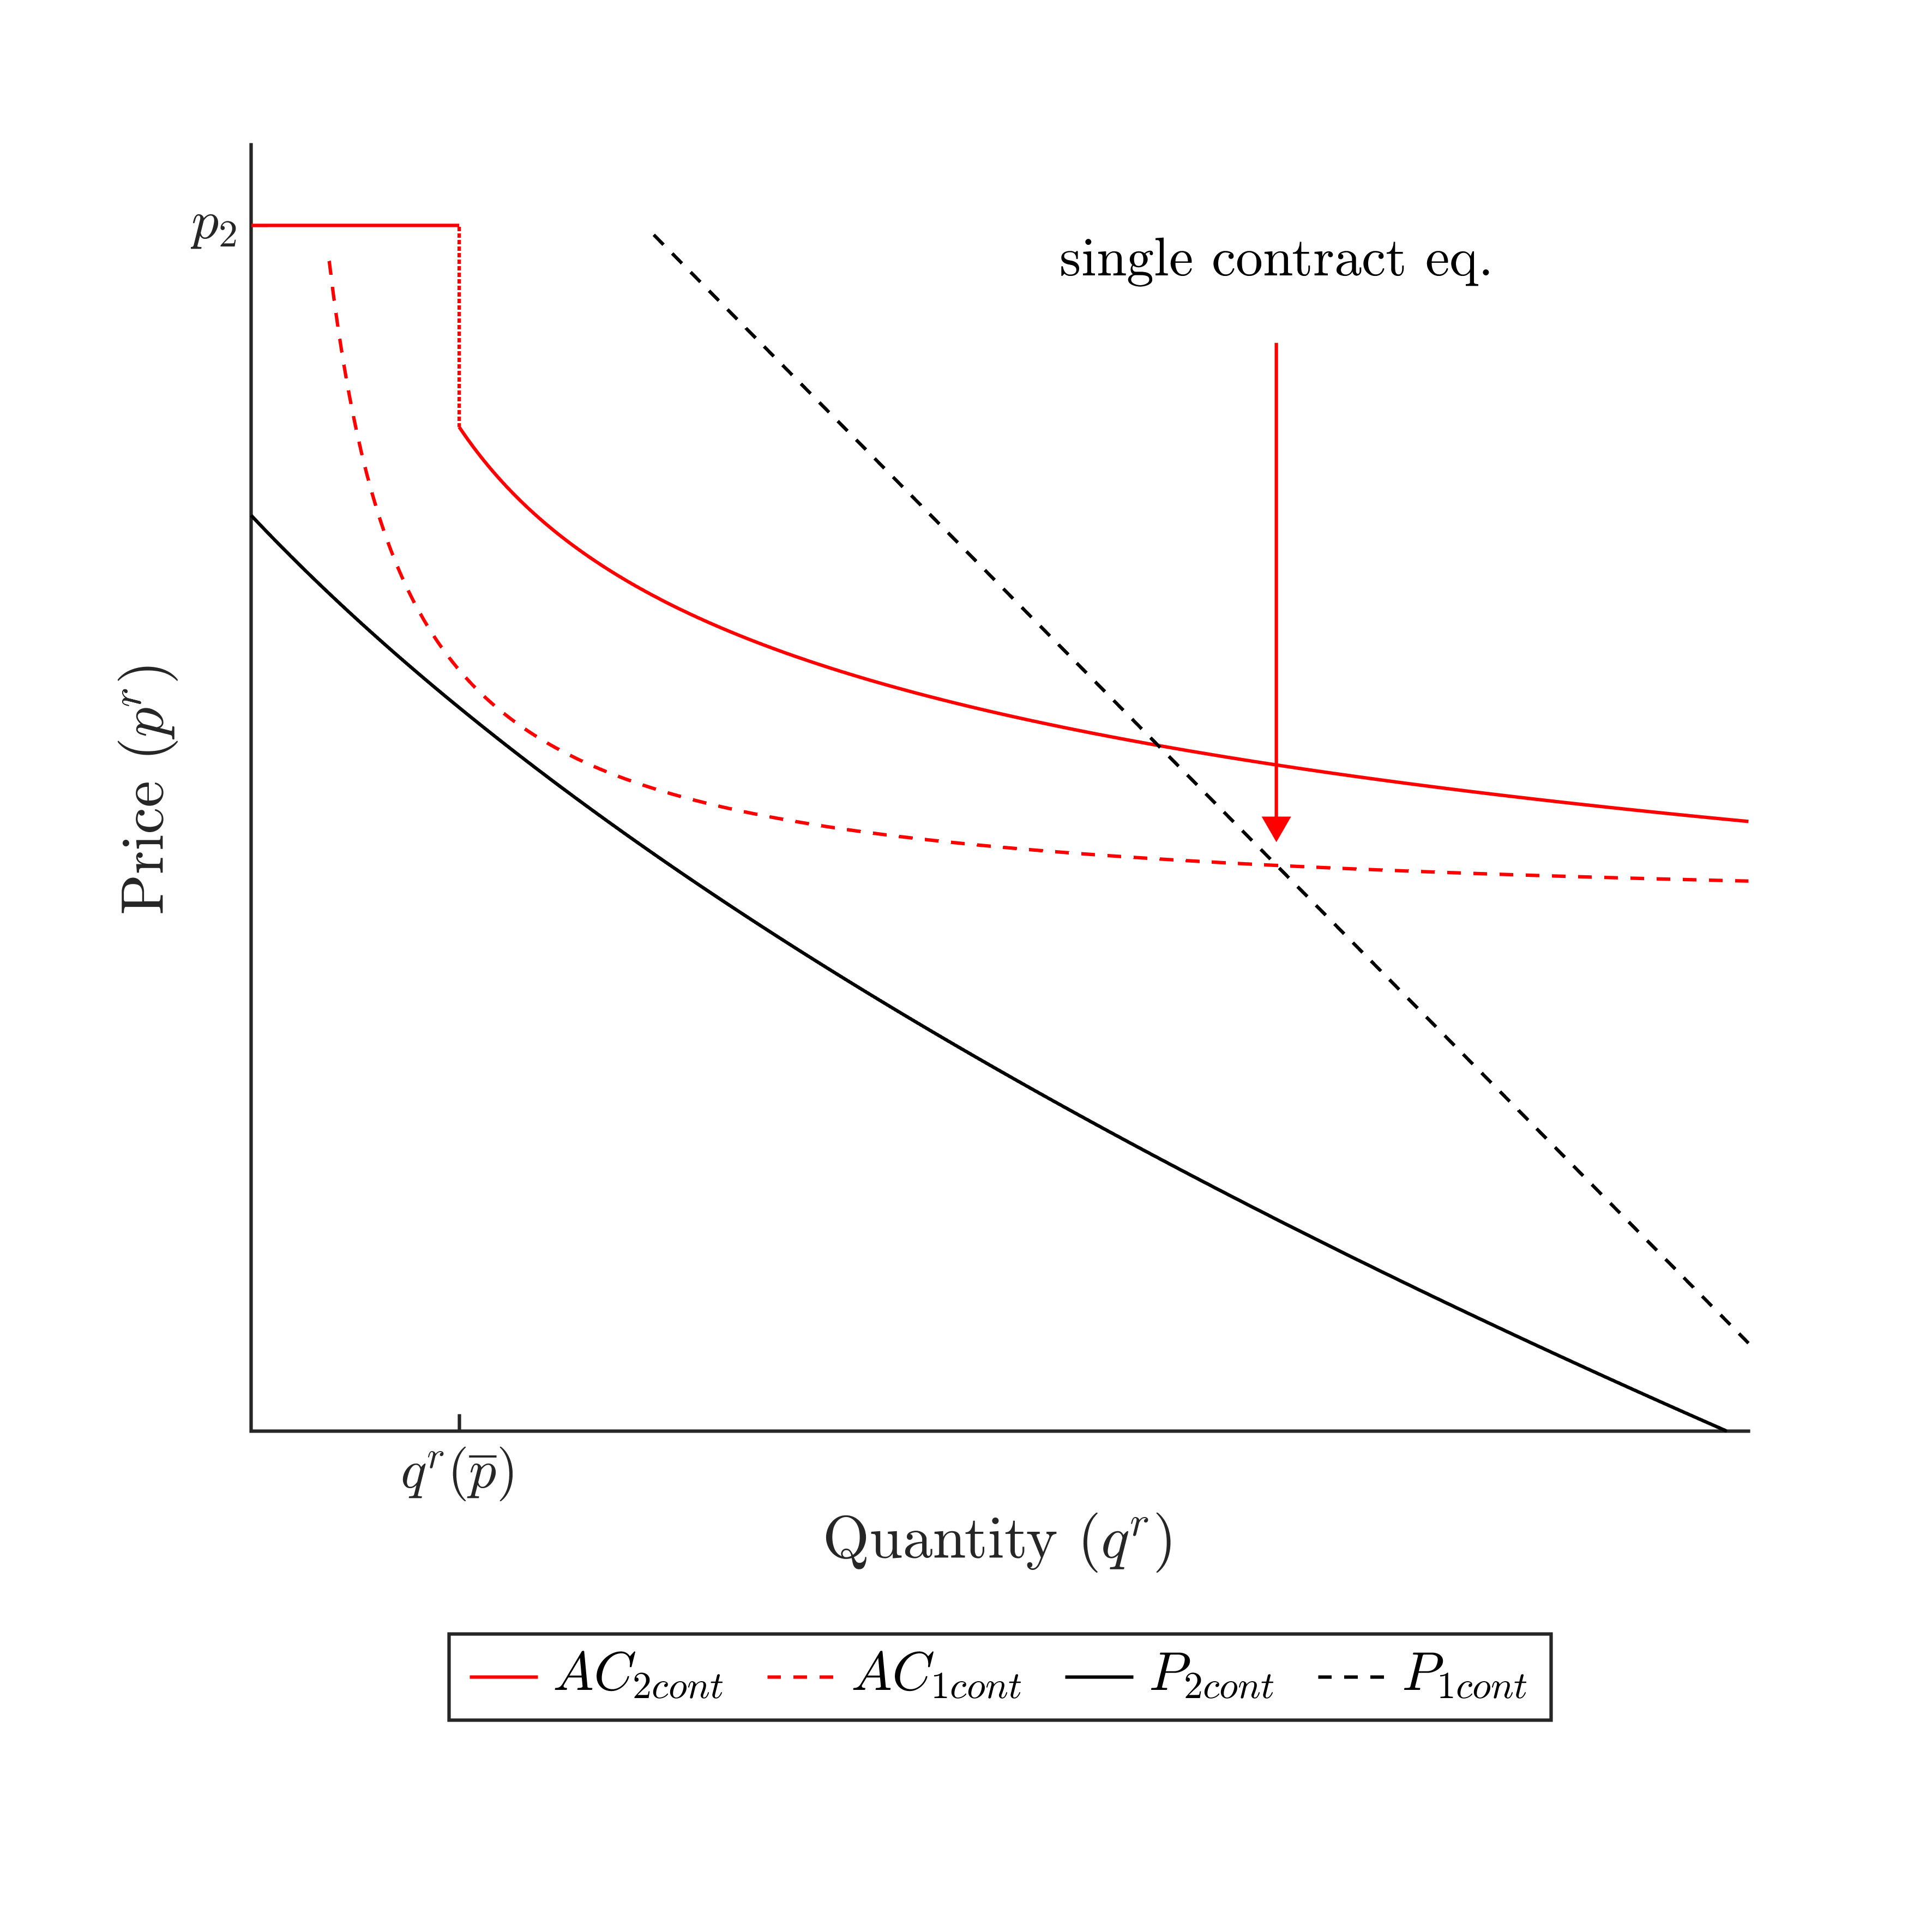
\includegraphics[width=1\linewidth]{figure/Exemple_Private_u_ddeAC_ppt.png}
\end{figure}
    
\end{frame}
% 
%%%%%%%%%%%%%%%%%%%%%%%%%%%%%%%%%%%%%%%%%%%%%%%%%%%%%%%%%%%%%%%%%%%%%%%%%%%%%%%%%%%%%%%%%%%%%%%%%%%%%%%%%%%%%%%%%%%%%%%%%%%%%%%%%%%%%%%%%%%%%%%%%%%%%%

\begin{frame}{Public firm price equilibrium}\label{RamseyOutside}

Assume general objective function $CS^r + (1+\lambda) \pi^r$ and linear pricing $p_r$.

\vfill

\begin{proposition}

Starting from $p_r = p_2$, the public firm has an incentive to introduce a fixed-price contract if $ W(\Omega_1) > \lambda q^r(p_2)$ holds.


\end{proposition}


\vfill

\begin{proposition}
 
With $\delta q$, the quantity deviations, the linear price of the fixed-price contract with the regulated monopoly solves the following modified Ramsey prices:
 

\begin{equation*}
      p_r \quad = \quad \;\underbrace{ \frac{\lambda}{1+\lambda} \frac{q^r}{\delta q^r}}_{\text{Ramsey term}} \quad + \quad \underbrace{p^w_1\frac{\delta q^r_1}{\delta q^r}+p^w_2\frac{\delta q^r_2}{\delta q^r}}_{\text{Multi. types}} \quad -  \;   \underbrace{\bigg. \Omega \bigg.}_{\text{foregone surplus}}  
\end{equation*}

\end{proposition}


\end{frame}
%%%%%%%%%%%%%%%%%%%%%%%%%%%%%%%%%%%%%%%%%%%%%%%%%%%%%%%%%%%%%%%%%%%%%%%%%%%%%%%%%%%%%%%%%%%%%%%%%%%%%%%%%%%%%%%%%%%%%%%%%%%%%%%%%%%%%%%%%%%%%%%%%%%%%%

% \begin{frame}{With the regulated monopoly }\label{RamseyMonopoly}


% \begin{itemize}
%     \item We assume that the public firm relies on two sources of financing:  \vfill
%     \begin{itemize}
%         \item The profit from the regulated fixed-price contract.  \vfill
%         \item Unitary tax $t$ levied on all electricity consumers. \vfill
%     \end{itemize}
% \end{itemize}

% \begin{result}

% \vspace{0.1cm}

% There exist some consumers who strictly prefer the FP contract. The full price ($p_r+t_r$) set by the firm solves the following:
 
% \begin{equation*}
%  P_r^{**} \; = p_r^{**} +t_r^{**} \;  = \;  \text{av.marg.cost} \; + \; \text{ramsey}  \; - \;   \underbrace{\bigg. \Omega \bigg.}_{\text{foregone CS}} \; - \;   \underbrace{ \bigg. T \bigg.}_{\text{levy effect}}  
% \end{equation*}

% \end{result}

% \begin{itemize}
%     \item  $T$ = marginal revenue of the tax from the private consumers
%     \item  $\Omega$ = welfare of the \textit{contract switchers}
% \end{itemize}




% \end{frame}

%%%%%%%%%%%%%%%%%%%%%%%%%%%%%%%%%%%%%%%%%%%%%%%%%%%%%%%%%%%%%%%%%%%%%%%%%%%%%%%%%%%%%%%%%%%%%%%%%%%%%%%%%%%%%%%%%%%%%%%%%%%%%%%%%%%%%%%%%%%%%%%%%%%%%%

\begin{frame}{Incentive for fixed-price contract}

\begin{figure}
    \centering
    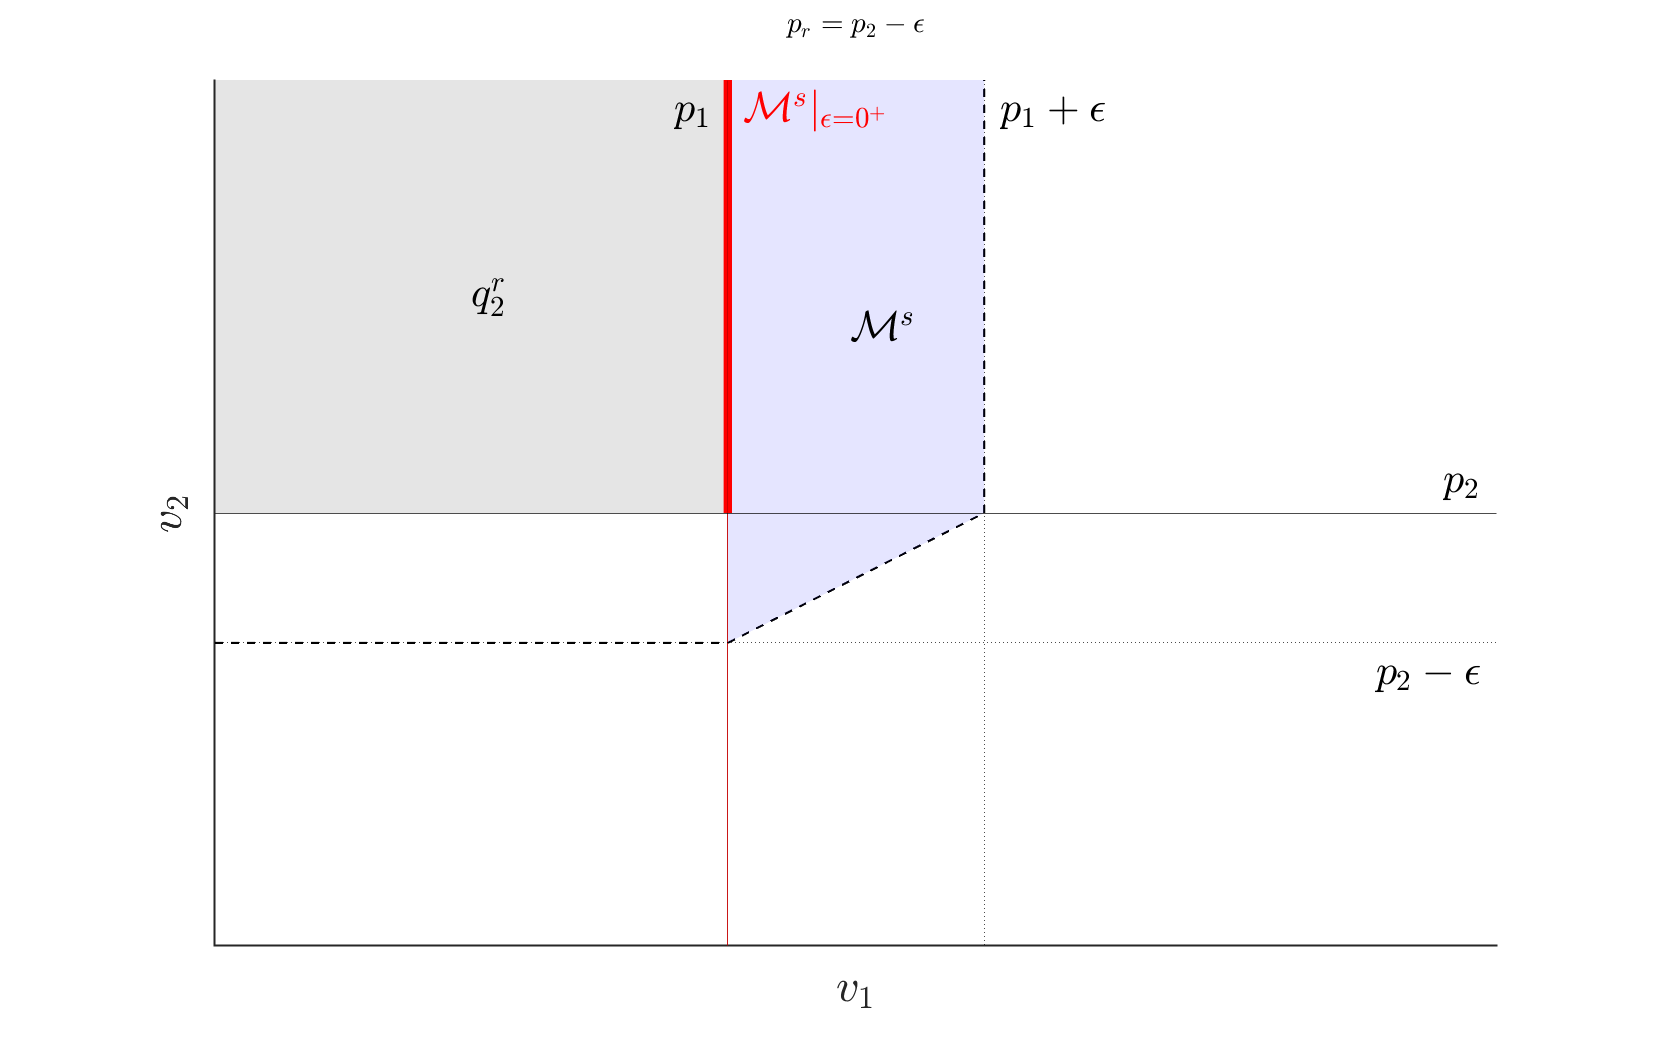
\includegraphics[width=1\linewidth]{figure/spot_demand_multi_sb_ppt_equil.png}
    \caption{Tradeoff for profitability of the public fixed-price contract.}
    \label{fig:spot_demand_multi_sb_ppt_equil}
\end{figure}
    
\end{frame}

%%%%%%%%%%%%%%%%%%%%%%%%%%%%%%%%%%%%%%%%%%%%%%%%%%%%%%%%%%%%%%%%%%%%%%%%%%%%%%%%%%%%%%%%%%%%%%%%%%%%%%%%%%%%%%%%%%%%%%%%%%%%%%%%%%%%%%%%%%%%%%%%%%%%%%

\begin{frame}{Illustration of $\Omega$}

\begin{figure}
    \centering
    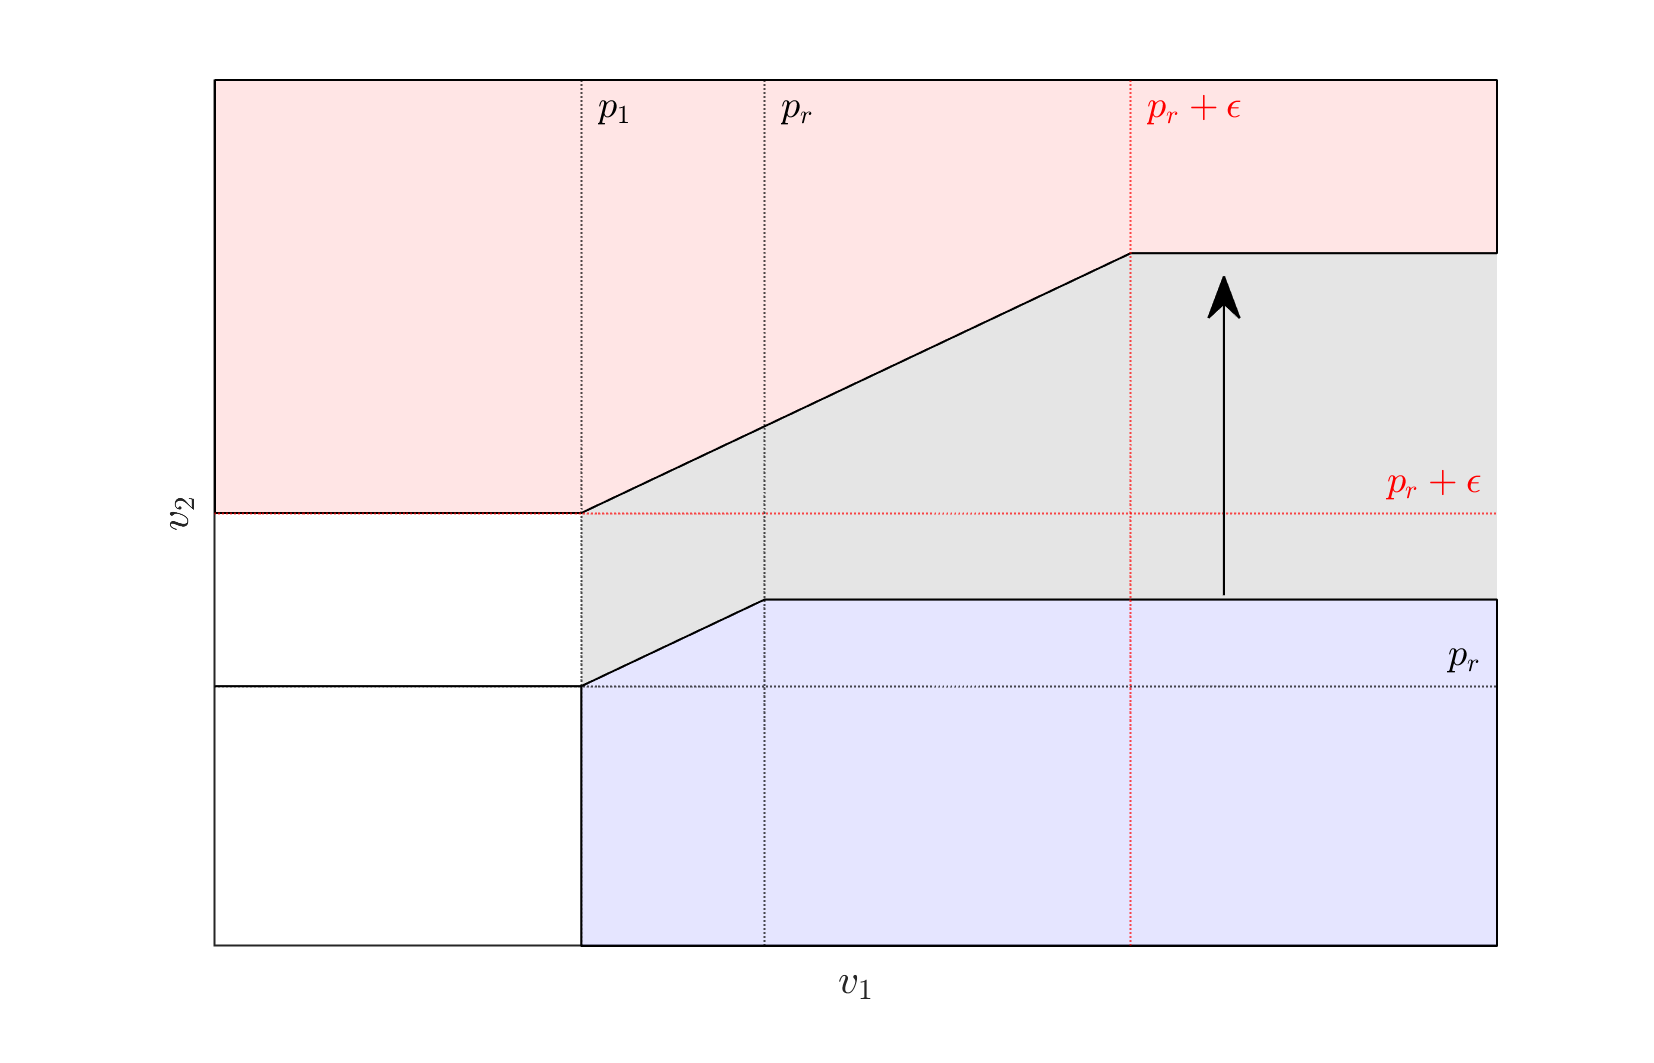
\includegraphics[width=1\linewidth]{figure/example_compstatpr_ppt.png}
    \caption{$\Omega$ captures the (marginal) consumer surplus lost to the private firms.}
    \label{fig:example_compstatpr_ppt}
\end{figure}
    
\end{frame}

%%%%%%%%%%%%%%%%%%%%%%%%%%%%%%%%%%%%%%%%%%%%%%%%%%%%%%%%%%%%%%%%%%%%%%%%%%%%%%%%%%%%%%%%%%%%%%%%%%%%%%%%%%%%%%%%%%%%%%%%%%%%%%%%%%%%%%%%%%%%%%%%%%%%%%

\section{Welfare Implications}

%%%%%%%%%%%%%%%%%%%%%%%%%%%%%%%%%%%%%%%%%%%%%%%%%%%%%%%%%%%%%%%%%%%%%%%%%%%%%%%%%%%%%%%%%%%%%%%%%%%%%%%%%%%%%%%%%%%%%%%%%%%%%%%%%%%%%%%%%%%%%%%%%%%%%%

\begin{frame}{Roadmap}
  \tableofcontents [sectionstyle=show/shaded,subsectionstyle=show/shaded]
\end{frame}

%%%%%%%%%%%%%%%%%%%%%%%%%%%%%%%%%%%%%%%%%%%%%%%%%%%%%%%%%%%%%%%%%%%%%%%%%%%%%%%%%%%%%%%%%%%%%%%%%%%%%%%%%%%%%%%%%%%%%%%%%%%%%%%%%%%%%%%%%%%%%%%%%%%%%%

\begin{frame}{Welfare comparison}


\begin{itemize}
   
    \item Only private firms: \boldrblue{ First-Best}. \vfill

    \item Public Firm + Private Firms + Consumer Choices \boldrblue{?} \vfill

    \item We compare the welfare with \boldrblue{a single contract} environment. \vfill

    \begin{itemize}
        \item We show that the \boldrblue{welfare can be ambiguous}. \vfill
        \item This is notably due to having \boldrblue{a lower fixed-price} compared to the single contract case.
    \end{itemize}
    
\end{itemize}
    
\end{frame}


\begin{frame}{Self-Selection Equilibrium vs. S.B. Linear Pricing FP Contract }

\begin{figure}
    \centering
    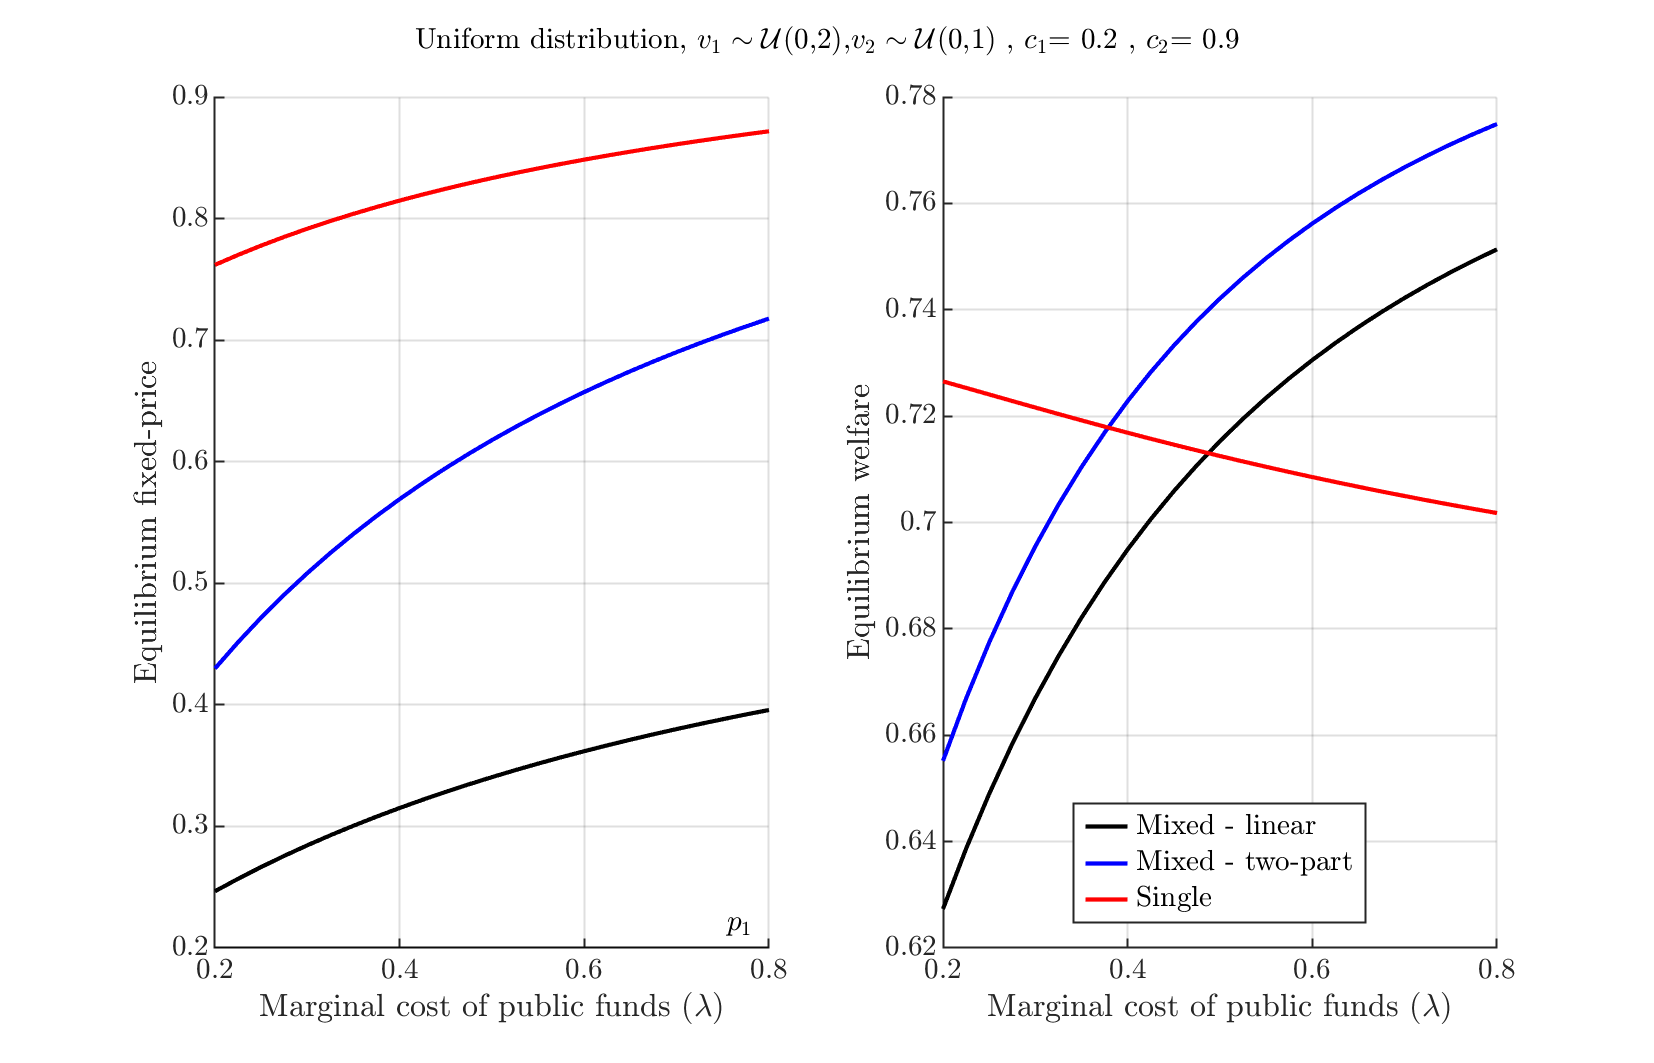
\includegraphics[width=0.9\linewidth]{figure/example_equ0_PublicFund_u.png}
        \caption{$W = CS + \Pi$.}
\end{figure}
    
\end{frame}


%%%%%%%%%%%%%%%%%%%%%%%%%%%%%%%%%%%%%%%%%%%%%%%%%%%%%%%%%%%%%%%%%%%%%%%%%%%%%%%%%%%%%%%%%%%%%%%%%%%%%%%%%%%%%%%%%%%%%%%%%%%%%%%%%%%%%%%%%%%%%%%%%%%%%%

\begin{frame}{Application - Equilibrium}

\begin{figure}
    \centering
    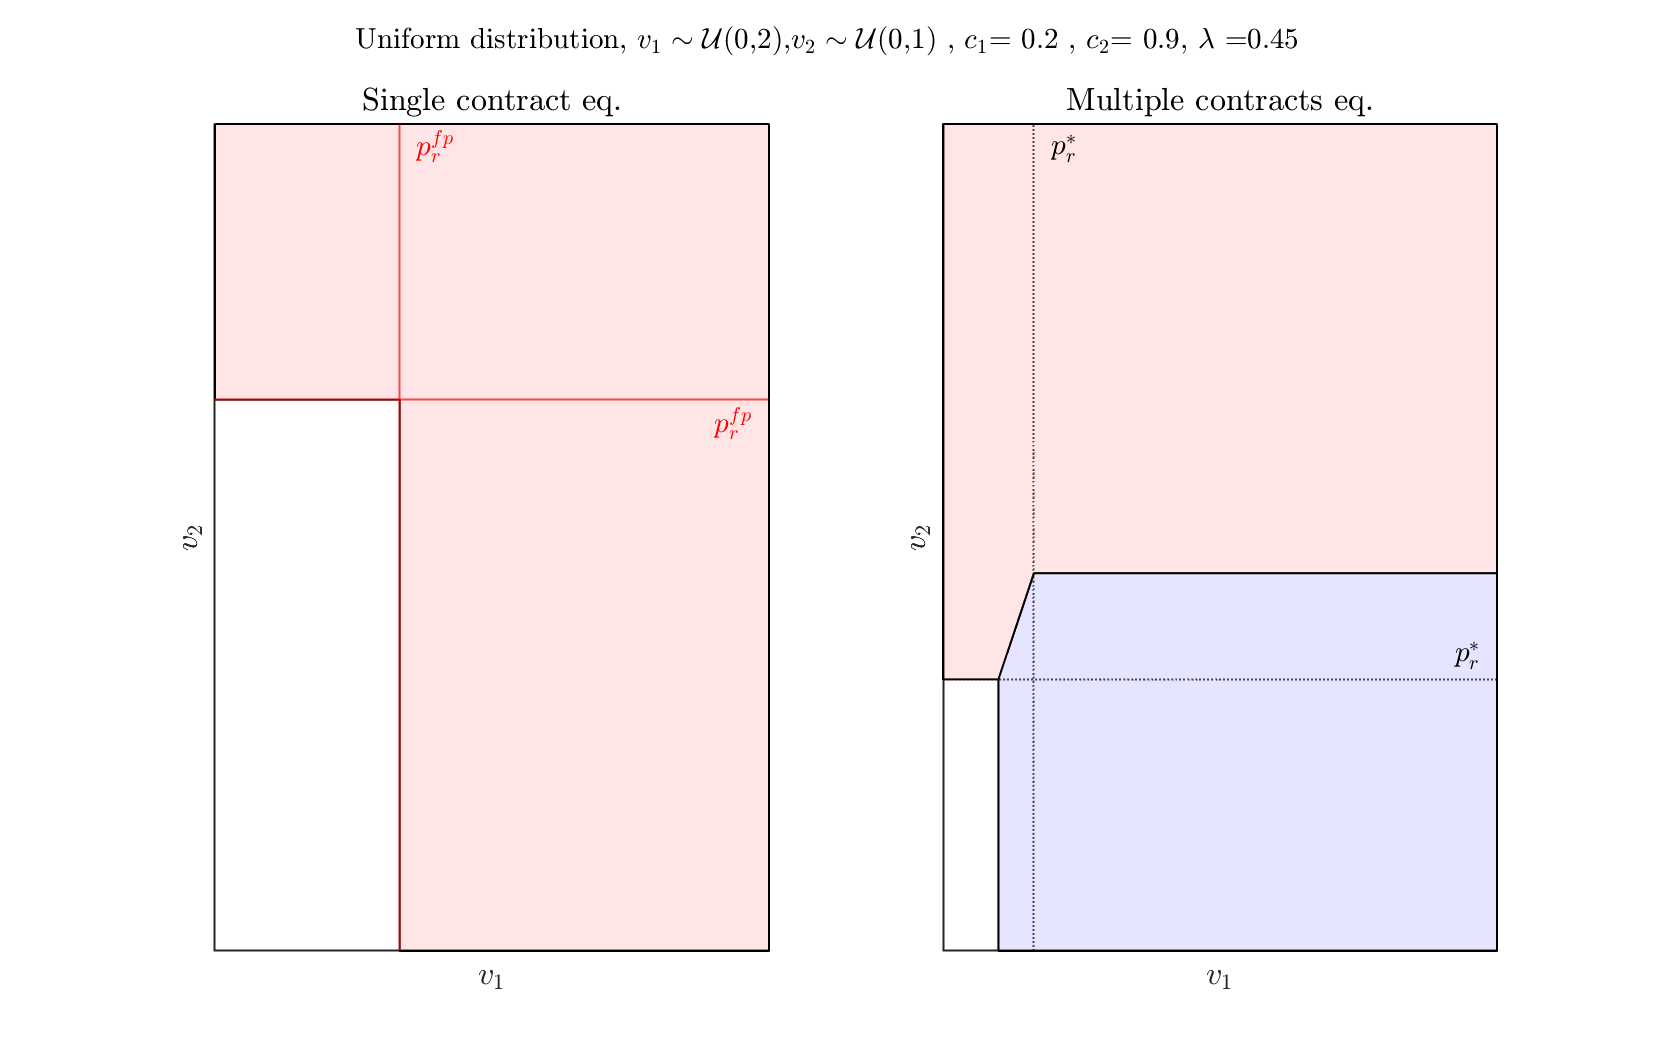
\includegraphics[width=0.95\linewidth]{figure/example_equ1_u.png}
\end{figure}
    
\end{frame}

%%%%%%%%%%%%%%%%%%%%%%%%%%%%%%%%%%%%%%%%%%%%%%%%%%%%%%%%%%%%%%%%%%%%%%%%%%%%%%%%%%%%%%%%%%%%%%%%%%%%%%%%%%%%%%%%%%%%%%%%%%%%%%%%%%%%%%%%%%%%%%%%%%%%%%


\begin{frame}{Application - Deadweight Loss in Period 1}

\begin{figure}
    \centering
    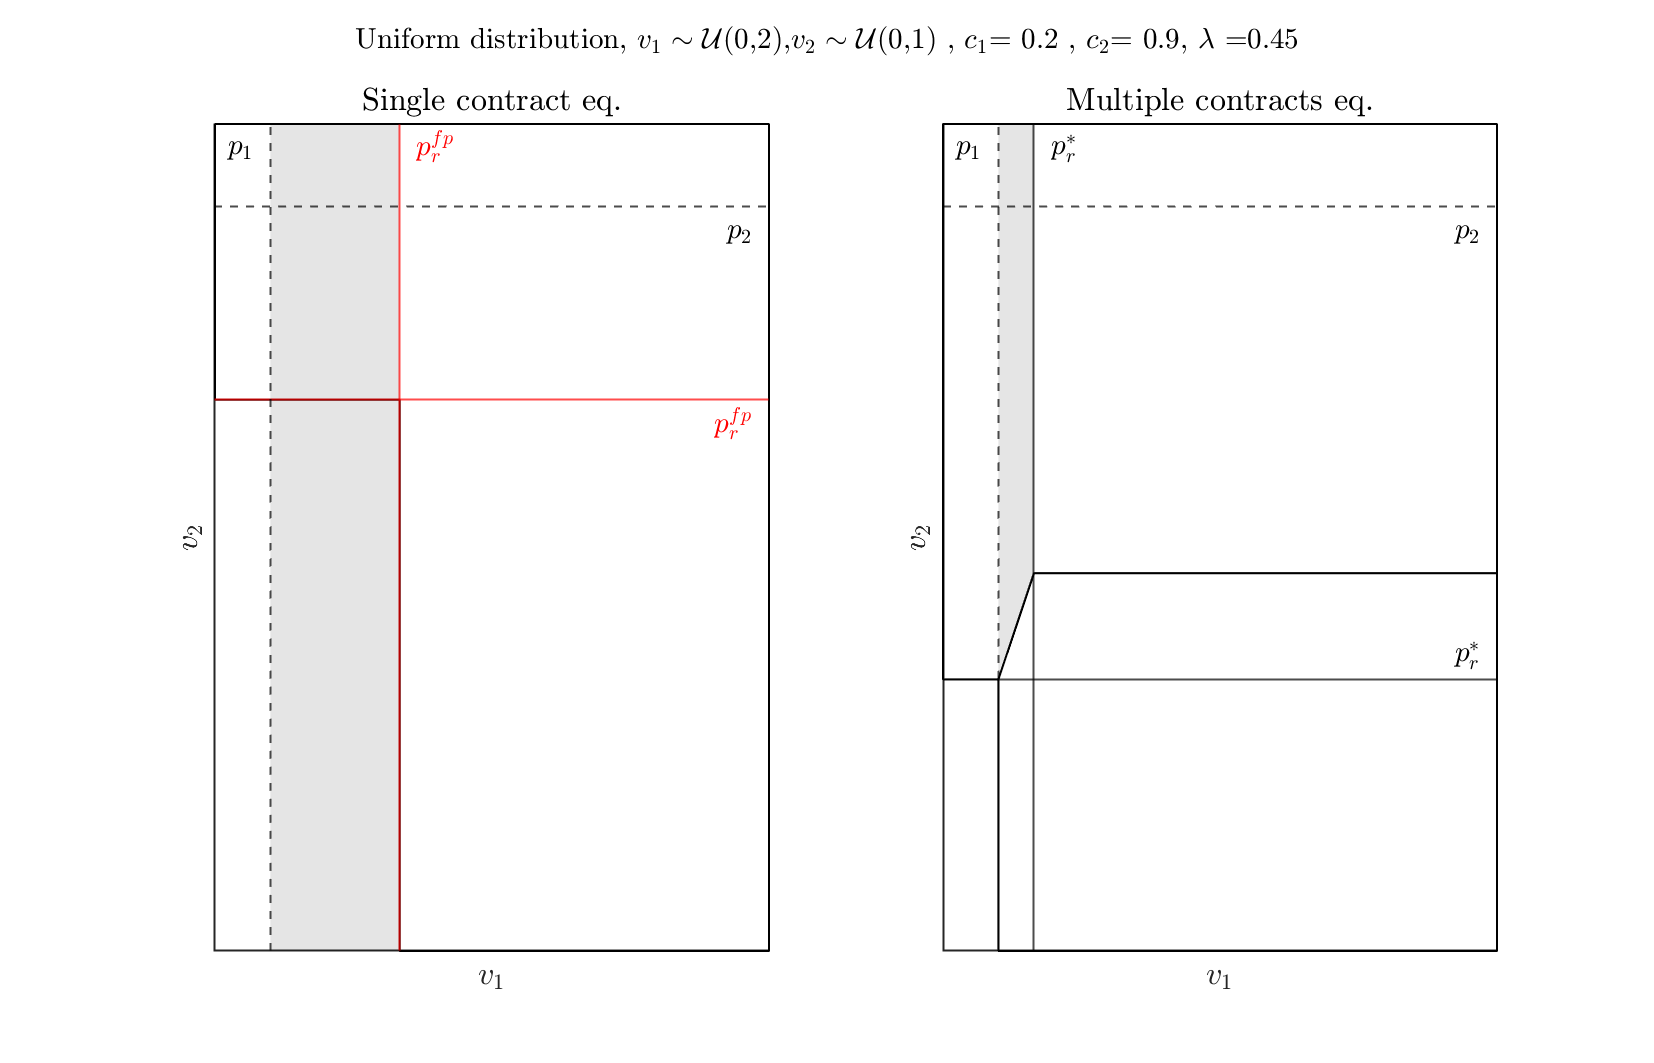
\includegraphics[width=0.95\linewidth]{figure/example_equ3_DW1_PublicFund_u.png}
\end{figure}
    
\end{frame}

%%%%%%%%%%%%%%%%%%%%%%%%%%%%%%%%%%%%%%%%%%%%%%%%%%%%%%%%%%%%%%%%%%%%%%%%%%%%%%%%%%%%%%%%%%%%%%%%%%%%%%%%%%%%%%%%%%%%%%%%%%%%%%%%%%%%%%%%%%%%%%%%%%%%%%


\begin{frame}{Application - Deadweight Loss in Period 2
}

\begin{figure}
    \centering
    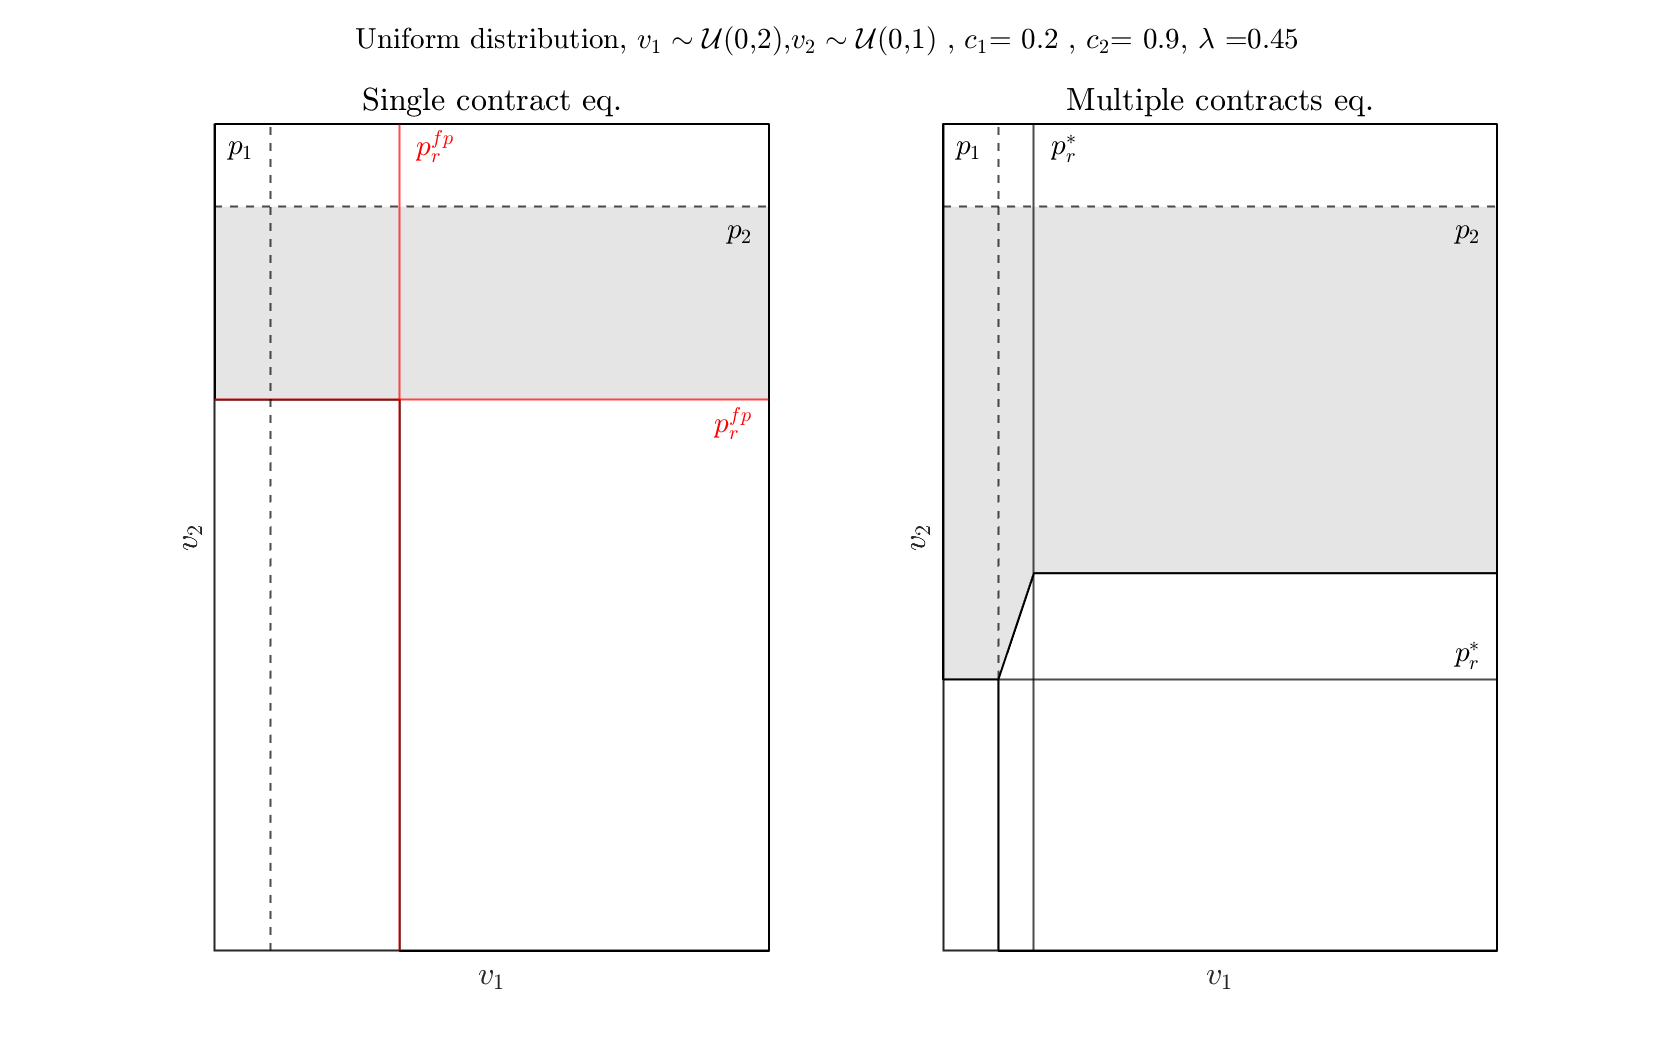
\includegraphics[width=0.95\linewidth]{figure/example_equ3_DW2_PublicFund_u.png}
\end{figure}
    
\end{frame}


%%%%%%%%%%%%%%%%%%%%%%%%%%%%%%%%%%%%%%%%%%%%%%%%%%%%%%%%%%%%%%%%%%%%%%%%%%%%%%%%%%%%%%%%%%%%%%%%%%%%%%%%%%%%%%%%%%%%%%%%%%%%%%%%%%%%%%%%%%%%%%%%%%%%%%

\begin{frame}{Application - Adverse selection at play}

\begin{figure}
    \centering
    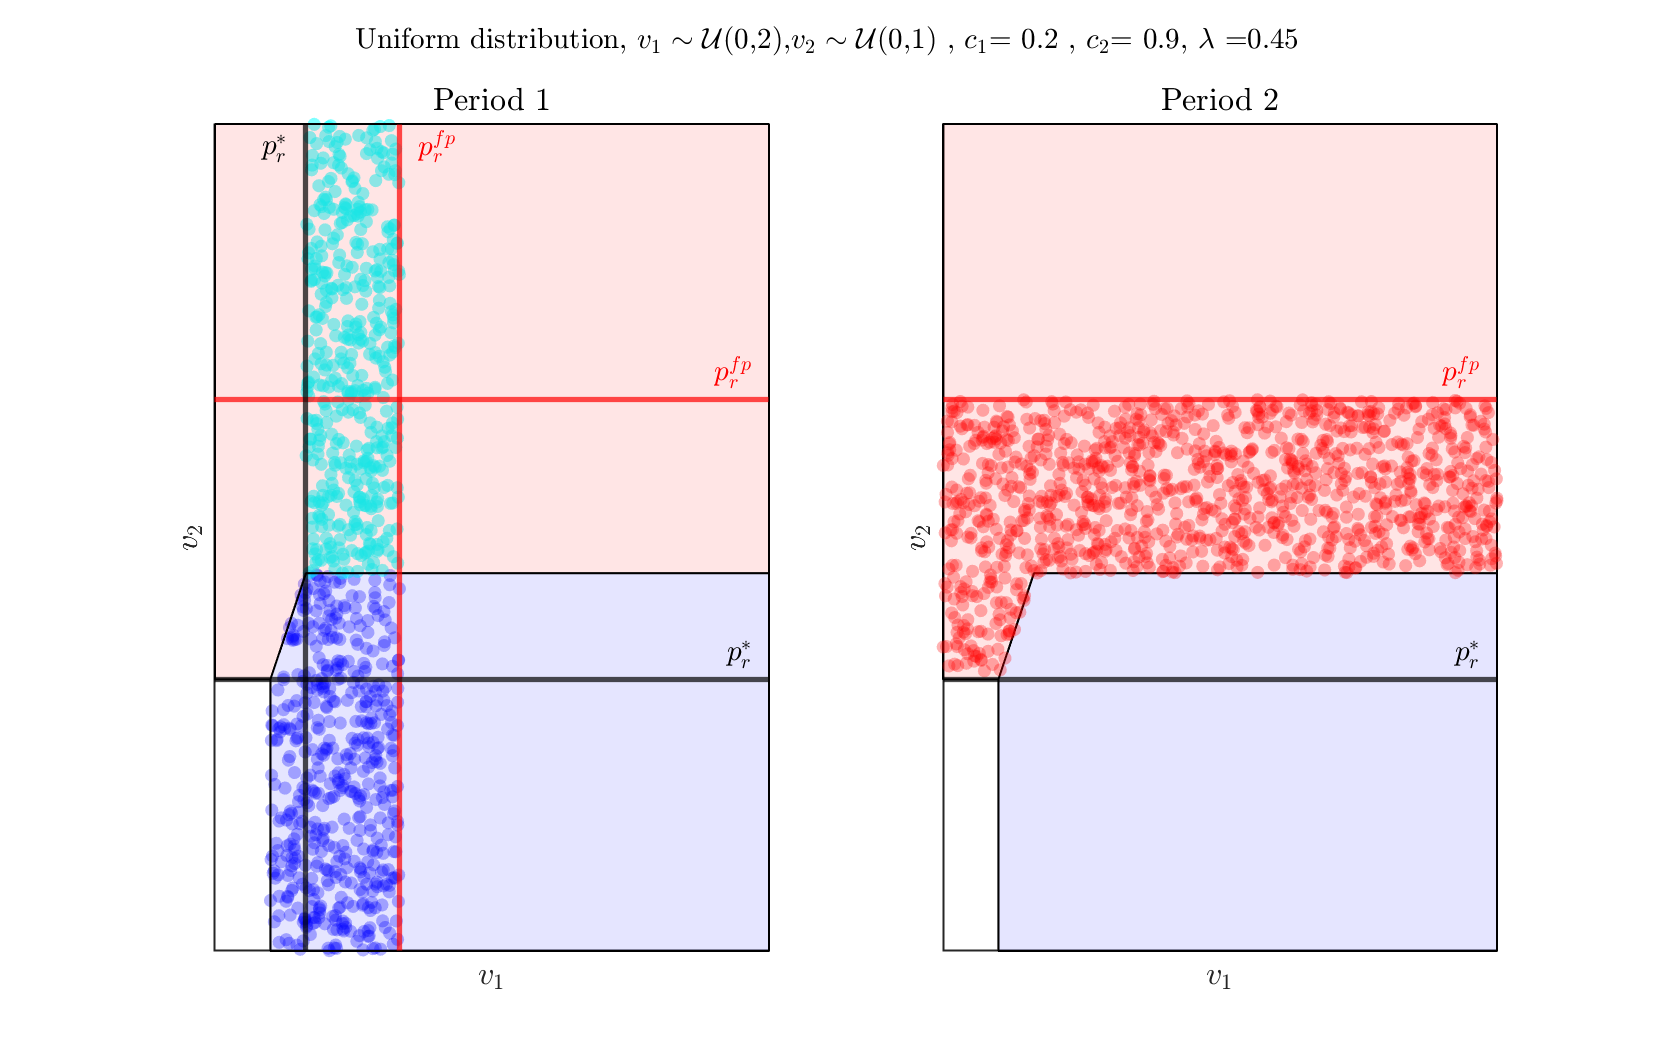
\includegraphics[width=0.95\linewidth]{figure/example_equ2_PublicFund_u.png}
\end{figure}
    
\end{frame}



%%%%%%%%%%%%%%%%%%%%%%%%%%%%%%%%%%%%%%%%%%%%%%%%%%%%%%%%%%%%%%%%%%%%%%%%%%%%%%%%%%%%%%%%%%%%%%%%%%%%%%%%%%%%%%%%%%%%%%%%%%%%%%%%%%%%%%%%%%%%%%%%%%%%%%


\section{Conclusion}



\begin{frame}{Conclusion}

\begin{itemize}
    \item The paper provides a novel framework describing the self-selection of electricity contracts by heterogeneous consumers.\vfill
    \item We characterize the contracts' price equilibrium in a specific retail market structure.\vfill
    \item We show that the coexistence of a public option with a private sector and self-selection from consumers can lead to low welfare due to adverse selection.\vfill
    \item The model provides some foundations for multiple extensions:
    \begin{itemize}
        \item Wholesale market to reflect clean technology adoption.
        \item Pricing topics (taxation, two-parts, screening).
        \item Consumer type (friction, ex ante technology choice).
        \item Redistributive issues.
    \end{itemize}
\end{itemize}
    
\end{frame}



% \end{document}


%%%%%%%%%%%%%%%%%%%%%%%%%%%%%%%%%%%%%%%%%%%%%%%%%%%%%%%%%%%%%%%%%%%%%%%%%%%%%%%%%%%%%%%%%%%%%%%%%%%%%%%%%%%%%%%%%%%%%%%%%%%%%%%%%%%%%%%%%%%%%%%%%%%%%%


\begin{frame}{}
  \centering {\Huge
  \emph{Thank you !}}
  
  \vspace{1cm}

  http://leopoldmonjoie.com/
\end{frame}


\newcounter{totalbeforeappendix}
\setcounter{totalbeforeappendix}{\value{framenumber}}
\addtocounter{totalbeforeappendix}{2} 
\addtocounter{framenumber}{-9}


\begin{frame}{Literature: Demand for contracts}\label{Lit_Conso}

\begin{itemize}
    \item \textbf{No theoretical foundation of self-selection in the power retail market}.

    \vfill
    
    \item Variation of an \boldrblue{exogenous share} of RTP consumers.
    \begin{itemize}
        \item Seminal paper: \cite{Borenstein2005b}, Technological cost \cite{Leautier2014},  Interactions with renewable technologies \cite{Ambec2021}, Risk aversion \cite{Boom2021}.
        \item \boldrblue{limits}: single period - homogenous consumers. 
    \end{itemize}

 \vfill

    \item \boldrblue{Empirical evidence} of self-selection with heterogeneous consumers
    \begin{itemize}
        \item Adverse selection \cite{Ito2023} Risk aversion \cite{Qiu2018} Behavioral bias \cite{Hortacsu2017,Fowlie2021}
        \item \boldrblue{limits}: focus on behavioral biais.
    \end{itemize}


\vfill
    \item Empirical evidence of RTP contracts.
    
    \begin{itemize}
        \item Effect of contract prices on consumption \cite{Fabra2021,Han2023,Enrich2024,Fu2024}, Redistributive effect \cite{Leslie2021, Levinson2022a, Cahana2023}
    \end{itemize}


     
    
\end{itemize}

\vfill

\hyperlink{FirstCont}{\beamergotobutton{Back}}

\end{frame}

%%%%%%%%%%%%%%%%%%%%%%%%%%%%%%%%%%%%%%%%%%%%%%%%%%%%%%%%%%%%%%%%%%%%%%%%%%%%%%%%%%%%%%%%%%%%%%%%%%%%%%%%%%%%%%%%%%%%%%%%%%%%%%%%%%%%%%%%%%%%%%%%%%%%%%

\begin{frame}{Literature: Retail competition}\label{Lit_Mkt1}
    
    
\begin{itemize}
    \item \textbf{Little attention on the competition in the retail market and contract equilibrium}.  
    
    \vfill

    \item Few empirical works on the benefit of retail competition \cite{Concettini2013}. Retailers acting as in Bertrand competition \cite{von2010electricity}
    
    \vfill

   \item Seminal papers \cite{joskow2006retail} and \cite{Borenstein2003}. \boldrblue{limits}: homogeneous consumers - simplified market structure.

\vfill

   \item  \boldrblue{Adverse selection} in retail electricity market
   
   \begin{itemize}
       \item Consumers deviation \cite{chao2013incentive}
       \item IC contracts and market equilibrium \cite{Astier2021}
   \end{itemize}

\vfill

    \item \boldrblue{Outside public option with incomplete information}
    \begin{itemize}
        \item In electricity markets with a regulated firm with redistributive preferences \cite{Martimort2020a} in a general setting \cite{Kang2023a}
    \end{itemize}


% \vfill

% \item Market power and price discrimination in retail electricity market \cite{byrne2022price}

\end{itemize}

\vfill



\hyperlink{SecondCont}{\beamergotobutton{Back}}

\end{frame}


%%%%%%%%%%%%%%%%%%%%%%%%%%%%%%%%%%%%%%%%%%%%%%%%%%%%%%%%%%%%%%%%%%%%%%%%%%%%%%%%%%%%%%%%%%%%%%%%%%%%%%%%%%%%%%%%%%%%%%%%%%%%%%%%%%%%%%%%%%%%%%%%%%%%%%

\begin{frame}{Literature: Other litterature }\label{Lit_Mkt2}
    
    
\begin{itemize}

   \item \textbf{Adverse Selection}
   \begin{itemize}
       \item Selection on the level and selection on the slope \cite{Einav2011,Einav2021}
       \item Empirical evidence for electricity contracts \cite{Ito2023}
   \end{itemize}


\vfill

   \item \textbf{Self-Selection}
    \begin{itemize}
        \item Roy Model \cite{Barro2013}
        \item Applied to Energy Efficiency \cite{Allcott2014}
    \end{itemize}

\vfill

   \item \textbf{Durable Goods}
   \begin{itemize}
       \item Household as production unit \cite{Becker1965}
       \item Applied to short-term/long-term decisions \cite{Feger2022} 
   \end{itemize}

\vfill

   \item \textbf{Competition for non-linear contracts}
   \begin{itemize}
       \item General setting \cite{Stole2007}
       \item Applied to insurance \cite{Rothschild1976,Dosis2022} 
   \end{itemize}
   
\vfill

   \item \textbf{Multidimensional Screening} \cite{Rochet1998}
   
\end{itemize}
\vfill

\hyperlink{SecondCont}{\beamergotobutton{Back}}

\end{frame}


%%%%%%%%%%%%%%%%%%%%%%%%%%%%%%%%%%%%%%%%%%%%%%%%%%%%%%%%%%%%%%%%%%%%%%%%%%%%%%%%%%%%%%%%%%%%%%%%%%%%%%%%%%%%%%%%%%%%%%%%%%%%%%%%%%%%%%%%%%%%%%%%%%%%%%
%%%%%%%%%%%%%%%%%%%%%%%%%%%%%%%%%%%%%%%%%%%%%%%%%%%%%%%%%%%%%%%%%%%%%%%%%%%%%%%%%%%%%%%%%%%%%%%%%%%%%%%%%%%%%%%%%%%%%%%%%%%%%%%%%%%%%%%%%%%%%%%%%%%%%%
%%%%%%%%%%%%%%%%%%%%%%%%%%%%%%%%%%%%%%%%%%%%%%%%%%%%%%%%%%%%%%%%%%%%%%%%%%%%%%%%%%%%%%%%%%%%%%%%%%%%%%%%%%%%%%%%%%%%%%%%%%%%%%%%%%%%%%%%%%%%%%%%%%%%%%

\section{Appendix}

\appendix

%%%%%%%%%%%%%%%%%%%%%%%%%%%%%%%%%%%%%%%%%%%%%%%%%%%%%%%%%%%%%%%%%%%%%%%%%%%%%%%%%%%%%%%%%%%%%%%%%%%%%%%%%%%%%%%%%%%%%%%%%%%%%%%%%%%%%%%%%%%%%%%%%%%%%%

\begin{frame}{Literature: Contracts in electricity market}\label{Lit_FB}

\begin{itemize}
    \item Peak Load Pricing Theory: Optimal investment in electricity markets requires short-term marginal cost pricing \cite{m1949tarification,joskow2007reliability}. \vfill

\item Contracts that approximate the first-best.
    \begin{itemize}
        \item  TOU and CPP / Demand Response / RTP \cite{Hinchberger2024}
    \end{itemize}

    \vfill

\item Real-time pricing (RTP)
    \begin{itemize}
        \item Seminal modeling papers comparing fixed-price contracts and RTP contracts with short-term and long-term interactions: \cite{Borenstein2003,Borenstein2005a,Borenstein2005b}
        \item Reduction of market power: \cite{Poletti2020}
        \item Reduction of pollution: \cite{Borenstein2021} 
        \item Interaction with renewable technology: \cite{Imelda2024}
        \item Interaction with decarbonization technologies: \cite{bailey2024electric}
    \end{itemize}
\end{itemize}

    \vfill
    
 \hyperlink{Motivations}{\beamergotobutton{Back}}
    
\end{frame}



%%%%%%%%%%%%%%%%%%%%%%%%%%%%%%%%%%%%%%%%%%%%%%%%%%%%%%%%%%%%%%%%%%%%%%%%%%%%%%%%%%%%%%%%%%%%%%%%%%%%%%%%%%%%%%%%%%%%%%%%%%%%%%%%%%%%%%%%%%%%%%%%%%%%%%



%%%%%%%%%%%%%%%%%%%%%%%%%%%%%%%%%%%%%%%%%%%%%%%%%%%%%%%%%%%%%%%%%%%%%%%%%%%%%%%%%%%%%%%%%%%%%%%%%%%%%%%%%%%%%%%%%%%%%%%%%%%%%%%%%%%%%%%%%%%%%%%%%%%%%%

\begin{frame}{Available technology and contract options}\label{options1}

\begin{columns}

\begin{column}{0.55\textwidth}  %%<--- here
    \begin{center}
\begin{figure}
    \centering
    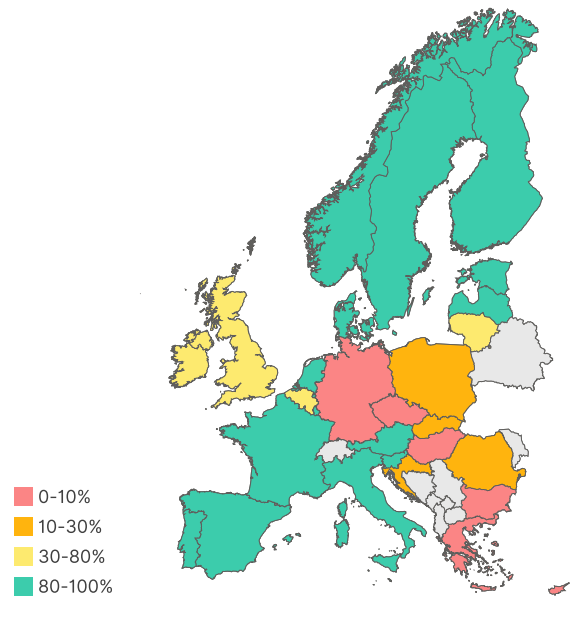
\includegraphics[width=0.75\linewidth]{figure/Smart_EU.PNG}
    \caption{Roll-out of smart meters among households \cite{ACER2024} }
    \label{fig:Smart_EU}
\end{figure}
     \end{center}
\end{column}
\begin{column}{0.50\textwidth}
\small	
 \boldrblue{20 EU countries out of 29} have regulated and non-regulated dynamic contract options for households \cite{ACER2024}
\hyperlink{ContractType}{\beamergotobutton{Table}},\hyperlink{USdata}{\beamergotobutton{US Data}},\hyperlink{options2}{\beamergotobutton{Details}},\hyperlink{UptakeContract2}{\beamergotobutton{Back }}
\hspace{2cm}
\end{column}
\end{columns}

\end{frame}


%%%%%%%%%%%%%%%%%%%%%%%%%%%%%%%%%%%%%%%%%%%%%%%%%%%%%%%%%%%%%%%%%%%%%%%%%%%%%%%%%%%%%%%%%%%%%%%%%%%%%%%%%%%%%%%%%%%%%%%%%%%%%%%%%%%%%%%%%%%%%%%%%%%%%%

\begin{frame}{Available technology and contract options}\label{options2}

% \begin{columns}

% \begin{column}{0.55\textwidth}  %%<--- here
%     \begin{center}
% \begin{figure}
%     \centering
%     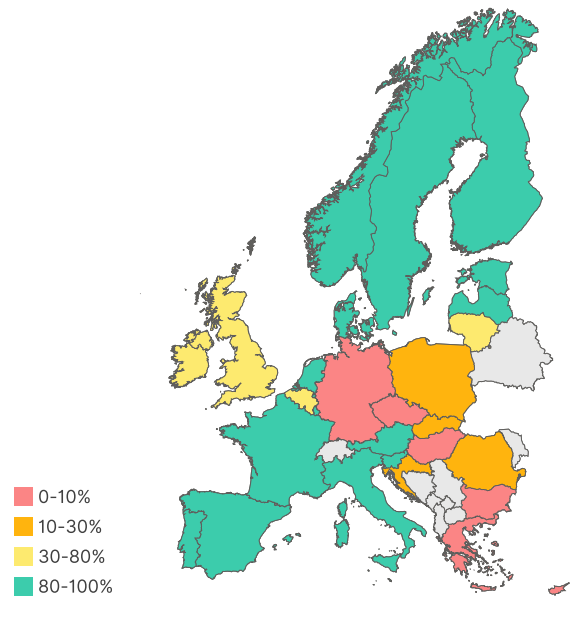
\includegraphics[width=0.75\linewidth]{figure/Smart_EU.PNG}
%     \caption{Roll-out of smart meters among households \cite{ACER2024} }
%     \label{fig:Smart_EU}
% \end{figure}
%      \end{center}
% \end{column}
% \begin{column}{0.50\textwidth}
% \small	
%  \boldrblue{20 EU countries out of 29} have regulated and non-regulated dynamic contract options for households \cite{ACER2024}

% \hspace{2cm}

\begin{figure}
    \centering
    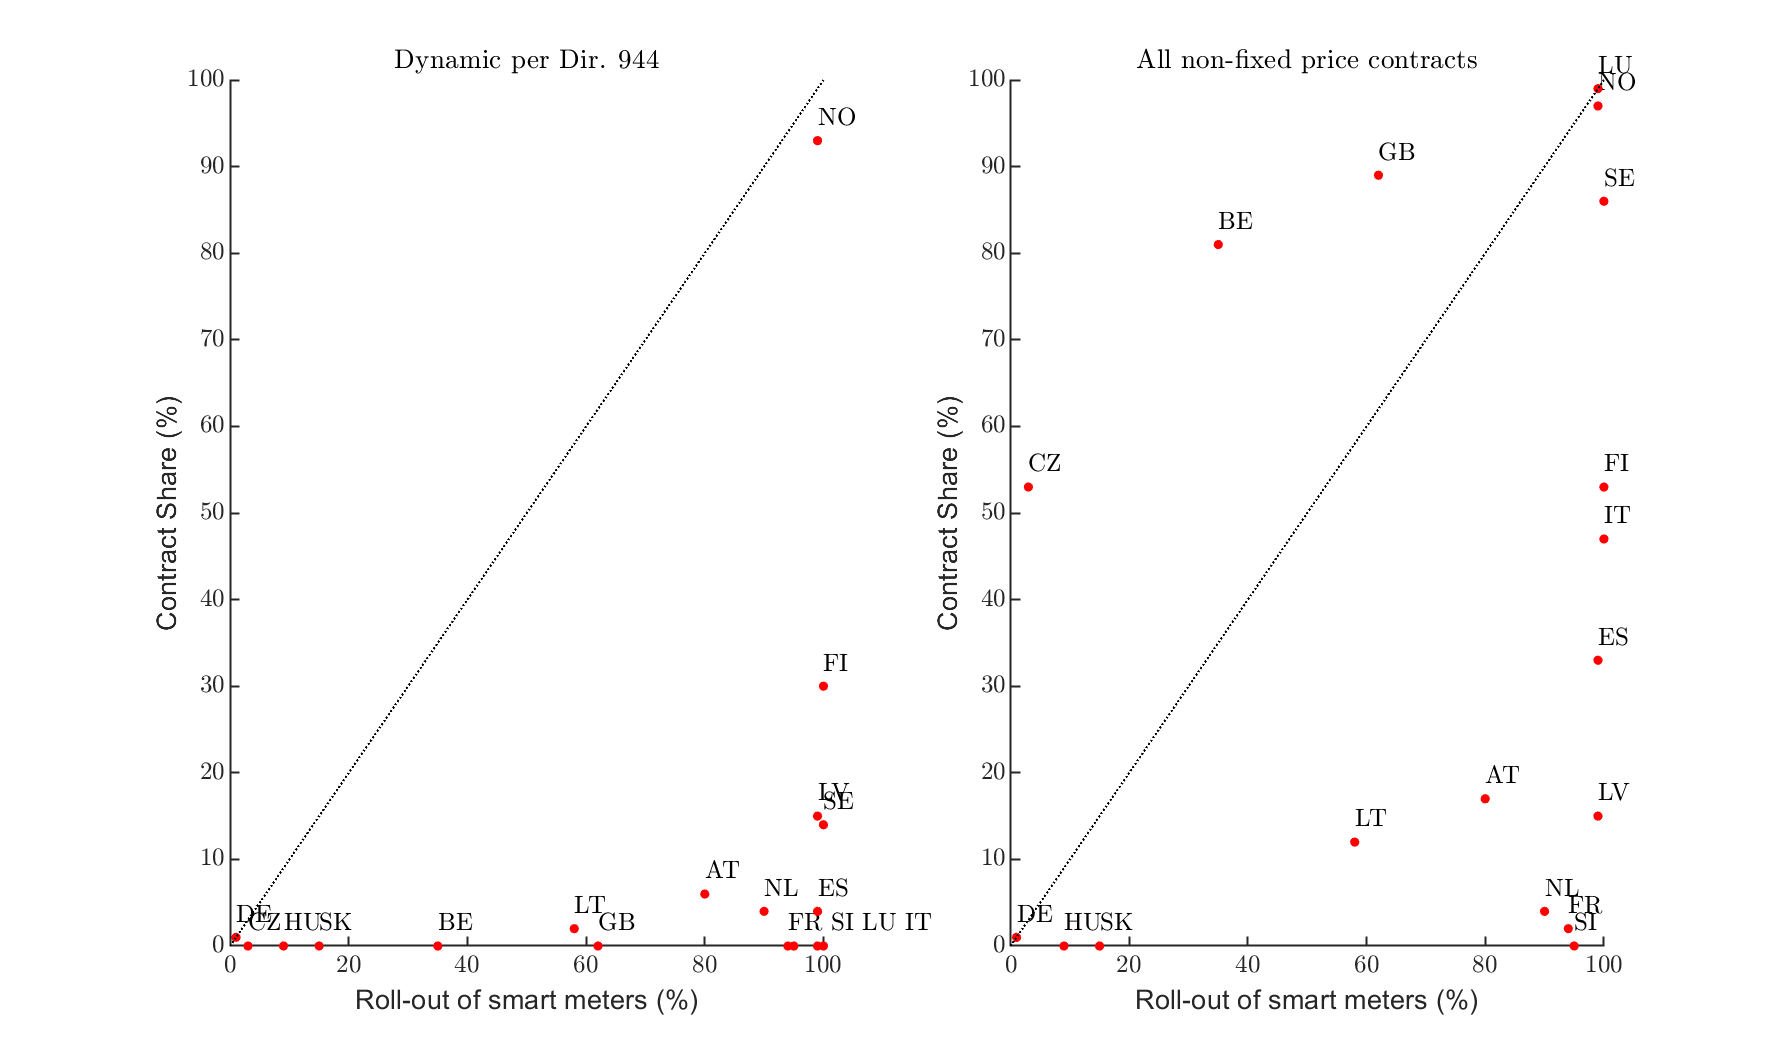
\includegraphics[width=1\linewidth]{figure/share_contract.PNG}
    \caption{Share of contract uptakes with respect to share of roll-out of smart meters among households (own calculation based on \cite{ACER2024}),\hyperlink{ContractType}{\beamergotobutton{Table}},\hyperlink{USdata}{\beamergotobutton{US Data}},\hyperlink{options1}{\beamergotobutton{Back}}}
    \label{fig:Smart_EU}
\end{figure}







% \end{column}
% \end{columns}



\end{frame}


%%%%%%%%%%%%%%%%%%%%%%%%%%
%%%%%%%%%%%%%%%%%%%%%%%%%%%%%%%%%%%%%%%%%%%%%%%%%%%%%%%%%%%%%%%%%%%%%%%%%%%%%%%%%%%%%%%%%%%%%%%%%%%%%%%%%%%%%%%%%%%%%%%%%%%%%%%%%%%%%%%%%%%%%%%%%%%%%%

\begin{frame}{Contract Options in the EU}\label{ContractType}

\begin{figure}
    \centering
    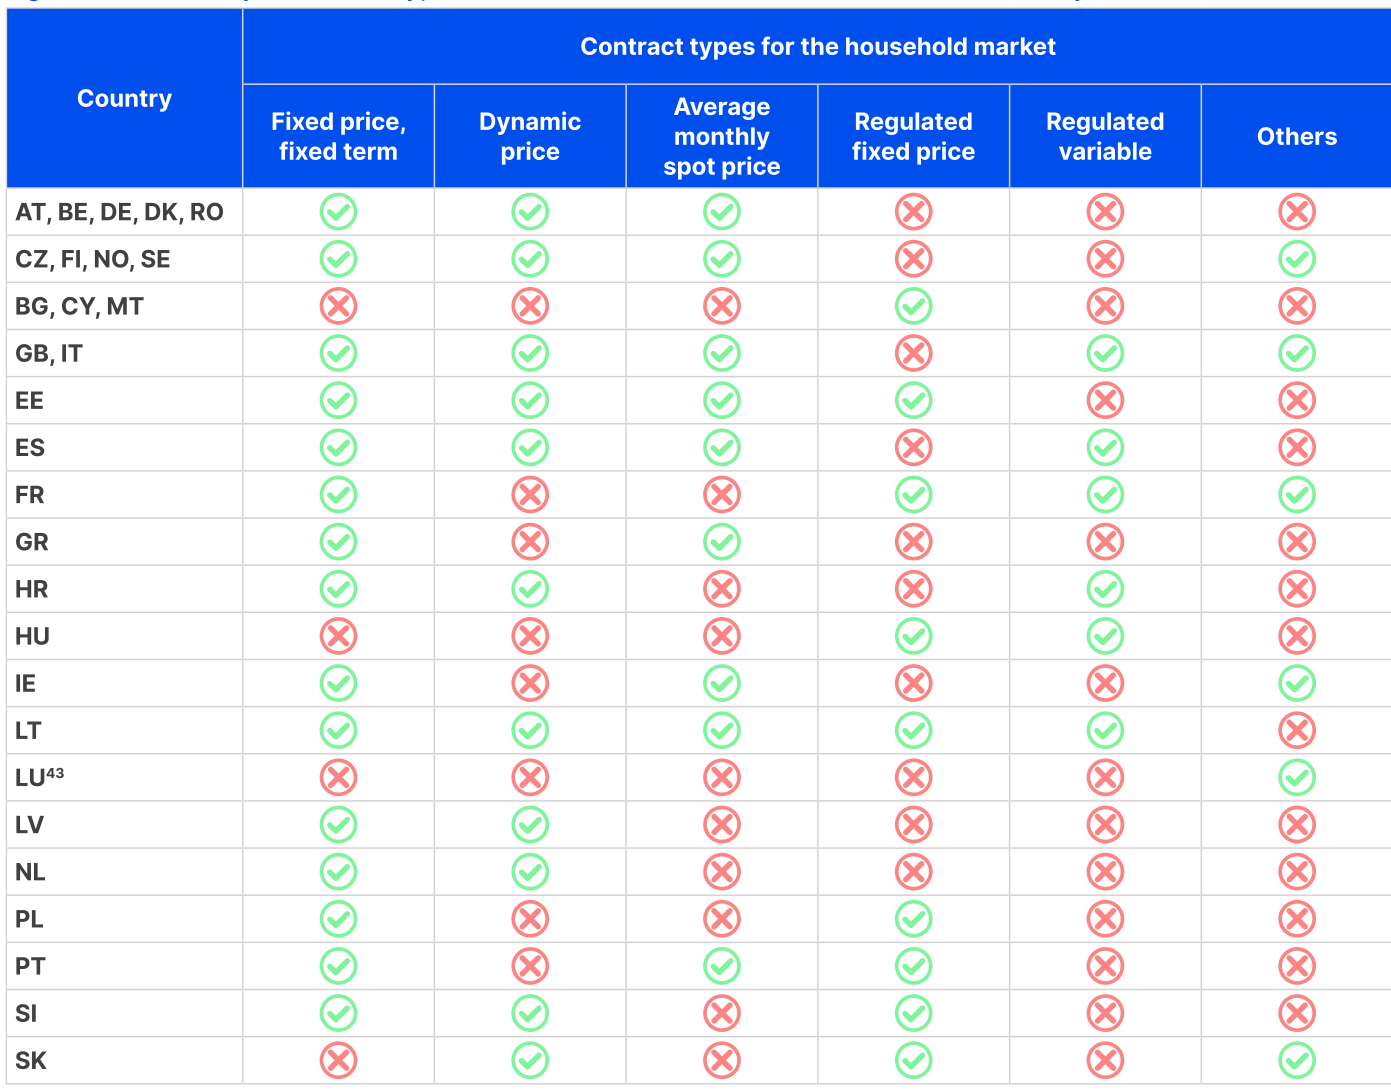
\includegraphics[width=0.8\linewidth]{figure/ContractType.PNG}
    \caption{Availability of different types of contracts to customers in the household electricity market in 2023 Country.\cite{ACER2024}  \hyperlink{options1}{\beamergotobutton{Back}} }
    \label{fig:ContractType}
\end{figure}
    
\end{frame}


%%%%%%%%%%%%%%%%%%%%%%%%%%%%%%%%%%%%%%%%%%%%%%%%%%%%%%%%%%%%%%%%%%%%%%%%%%%%%%%%%%%%%%%%%%%%%%%%%%%%%%%%%%%%%%%%%%%%%%%%%%%%%%%%%%%%%%%%%%%%%%%%%%%%%%

\begin{frame}{US Data}\label{USdata}

\begin{figure}
    \centering
    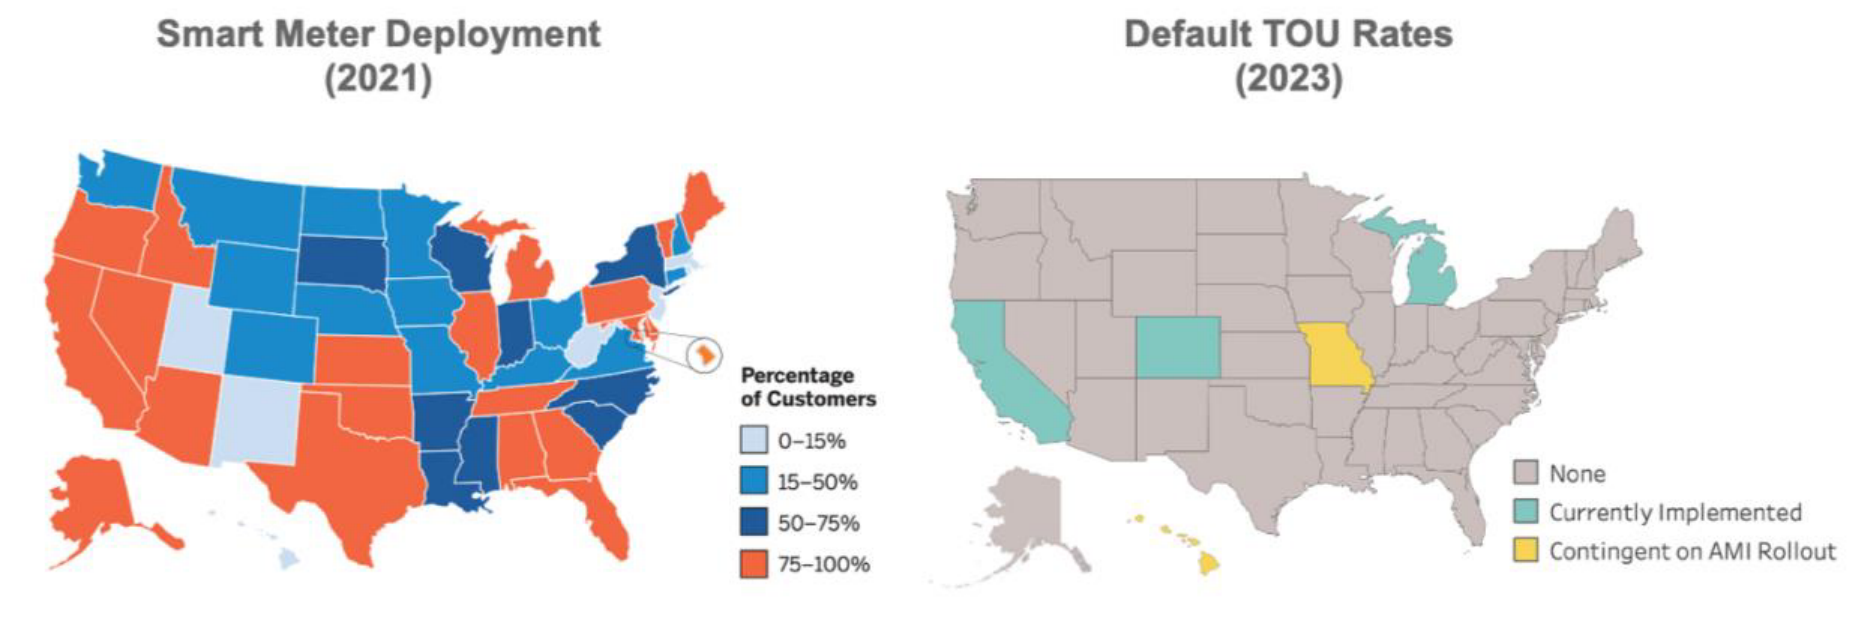
\includegraphics[width=1\linewidth]{figure/FP_Smart_US.PNG}
    \caption{Smart meter deployment among US households (left) and default TOU rate adoption (right). Default TOU rates are shown for each state's largest distribution utility. \cite{Turk2024}  \hyperlink{options1}{\beamergotobutton{Back}} }
    \label{fig:FP_Smart_US}
\end{figure}
    
\end{frame}

%%%%%%%%%%%%%%%%%%%%%%%%%%%%%%%%%%%%%%%%%%%%%%%%%%%%%%%%%%%%%%%%%%%%%%%%%%%%%%%%%%%%%%%%%%%%%%%%%%%%%%%%%%%%%%%%%%%%%%%%%%%%%%%%%%%%%%%%%%%%%%%%%%%%%%



\bibliography{bib}

\end{document}
